\documentclass[twoside]{book}

% Packages required by doxygen
\usepackage{fixltx2e}
\usepackage{calc}
\usepackage{doxygen}
\usepackage[export]{adjustbox} % also loads graphicx
\usepackage{graphicx}
\usepackage[utf8]{inputenc}
\usepackage{makeidx}
\usepackage{multicol}
\usepackage{multirow}
\PassOptionsToPackage{warn}{textcomp}
\usepackage{textcomp}
\usepackage[nointegrals]{wasysym}
\usepackage[table]{xcolor}

% Font selection
\usepackage[T1]{fontenc}
\usepackage[scaled=.90]{helvet}
\usepackage{courier}
\usepackage{amssymb}
\usepackage{sectsty}
\renewcommand{\familydefault}{\sfdefault}
\allsectionsfont{%
  \fontseries{bc}\selectfont%
  \color{darkgray}%
}
\renewcommand{\DoxyLabelFont}{%
  \fontseries{bc}\selectfont%
  \color{darkgray}%
}
\newcommand{\+}{\discretionary{\mbox{\scriptsize$\hookleftarrow$}}{}{}}

% Page & text layout
\usepackage{geometry}
\geometry{%
  a4paper,%
  top=2.5cm,%
  bottom=2.5cm,%
  left=2.5cm,%
  right=2.5cm%
}
\tolerance=750
\hfuzz=15pt
\hbadness=750
\setlength{\emergencystretch}{15pt}
\setlength{\parindent}{0cm}
\setlength{\parskip}{3ex plus 2ex minus 2ex}
\makeatletter
\renewcommand{\paragraph}{%
  \@startsection{paragraph}{4}{0ex}{-1.0ex}{1.0ex}{%
    \normalfont\normalsize\bfseries\SS@parafont%
  }%
}
\renewcommand{\subparagraph}{%
  \@startsection{subparagraph}{5}{0ex}{-1.0ex}{1.0ex}{%
    \normalfont\normalsize\bfseries\SS@subparafont%
  }%
}
\makeatother

% Headers & footers
\usepackage{fancyhdr}
\pagestyle{fancyplain}
\fancyhead[LE]{\fancyplain{}{\bfseries\thepage}}
\fancyhead[CE]{\fancyplain{}{}}
\fancyhead[RE]{\fancyplain{}{\bfseries\leftmark}}
\fancyhead[LO]{\fancyplain{}{\bfseries\rightmark}}
\fancyhead[CO]{\fancyplain{}{}}
\fancyhead[RO]{\fancyplain{}{\bfseries\thepage}}
\fancyfoot[LE]{\fancyplain{}{}}
\fancyfoot[CE]{\fancyplain{}{}}
\fancyfoot[RE]{\fancyplain{}{\bfseries\scriptsize Generated by Doxygen }}
\fancyfoot[LO]{\fancyplain{}{\bfseries\scriptsize Generated by Doxygen }}
\fancyfoot[CO]{\fancyplain{}{}}
\fancyfoot[RO]{\fancyplain{}{}}
\renewcommand{\footrulewidth}{0.4pt}
\renewcommand{\chaptermark}[1]{%
  \markboth{#1}{}%
}
\renewcommand{\sectionmark}[1]{%
  \markright{\thesection\ #1}%
}

% Indices & bibliography
\usepackage{natbib}
\usepackage[titles]{tocloft}
\setcounter{tocdepth}{3}
\setcounter{secnumdepth}{5}
\makeindex

% Hyperlinks (required, but should be loaded last)
\usepackage{ifpdf}
\ifpdf
  \usepackage[pdftex,pagebackref=true]{hyperref}
\else
  \usepackage[ps2pdf,pagebackref=true]{hyperref}
\fi
\hypersetup{%
  colorlinks=true,%
  linkcolor=blue,%
  citecolor=blue,%
  unicode%
}

% Custom commands
\newcommand{\clearemptydoublepage}{%
  \newpage{\pagestyle{empty}\cleardoublepage}%
}

\usepackage{caption}
\captionsetup{labelsep=space,justification=centering,font={bf},singlelinecheck=off,skip=4pt,position=top}

%===== C O N T E N T S =====

\begin{document}

% Titlepage & ToC
\hypersetup{pageanchor=false,
             bookmarksnumbered=true,
             pdfencoding=unicode
            }
\pagenumbering{alph}
\begin{titlepage}
\vspace*{7cm}
\begin{center}%
{\Large Eigen\+Faces \\[1ex]\large v0.\+1 }\\
\vspace*{1cm}
{\large Generated by Doxygen 1.8.13}\\
\end{center}
\end{titlepage}
\clearemptydoublepage
\pagenumbering{roman}
\tableofcontents
\clearemptydoublepage
\pagenumbering{arabic}
\hypersetup{pageanchor=true}

%--- Begin generated contents ---
\chapter{C\+H\+A\+N\+G\+E\+L\+OG}
\label{md__f_1__git_hub__projects__asdecalidad-1_website_src_website_bower_components_bootstrap__c_h_a_n_g_e_l_o_g}
\Hypertarget{md__f_1__git_hub__projects__asdecalidad-1_website_src_website_bower_components_bootstrap__c_h_a_n_g_e_l_o_g}
Bootstrap uses \href{https://github.com/blog/1547-release-your-software}{\tt Git\+Hub\textquotesingle{}s Releases feature} for its changelogs.

See \href{https://github.com/twbs/bootstrap/releases}{\tt the Releases section of our Git\+Hub project} for changelogs for each release version of Bootstrap.

Release announcement posts on \href{http://blog.getbootstrap.com}{\tt the official Bootstrap blog} contain summaries of the most noteworthy changes made in each release. 
\chapter{I\+S\+S\+U\+E\+\_\+\+T\+E\+M\+P\+L\+A\+TE}
\label{md__f_1__git_hub__projects__asdecalidad-1_website_src_website_bower_components_bootstrap__i_s_s_u_e__t_e_m_p_l_a_t_e}
\Hypertarget{md__f_1__git_hub__projects__asdecalidad-1_website_src_website_bower_components_bootstrap__i_s_s_u_e__t_e_m_p_l_a_t_e}
Before opening an issue\+:


\begin{DoxyItemize}
\item \href{https://github.com/twbs/bootstrap/issues?utf8=%E2%9C%93&q=is%3Aissue}{\tt Search for duplicate or closed issues}
\item \href{http://validator.w3.org/nu/}{\tt Validate} and \href{https://github.com/twbs/bootlint#in-the-browser}{\tt lint} any H\+T\+ML to avoid common problems
\item Prepare a \href{https://css-tricks.com/reduced-test-cases/}{\tt reduced test case} for any bugs
\item Read the https\+://github.com/twbs/bootstrap/blob/master/\+C\+O\+N\+T\+R\+I\+B\+U\+T\+I\+N\+G.\+md \char`\"{}contributing guidelines\char`\"{}
\end{DoxyItemize}

When asking general \char`\"{}how to\char`\"{} questions\+:


\begin{DoxyItemize}
\item Please do not open an issue here
\item Instead, ask for help on \href{https://github.com/twbs/bootstrap/blob/master/README.md#community}{\tt Stack\+Overflow, I\+RC, or Slack}
\end{DoxyItemize}

When reporting a bug, include\+:


\begin{DoxyItemize}
\item Operating system and version (Windows, Mac OS X, Android, i\+OS, Win10 Mobile)
\item Browser and version (Chrome, Firefox, Safari, IE, MS Edge, Opera 15+, Android Browser)
\item Reduced test cases and potential fixes using \href{https://jsbin.com}{\tt JS Bin}
\end{DoxyItemize}

When suggesting a feature, include\+:


\begin{DoxyItemize}
\item As much detail as possible for what we should add and why it\textquotesingle{}s important to Bootstrap
\item Relevant links to prior art, screenshots, or live demos whenever possible 
\end{DoxyItemize}
\chapter{\mbox{[}Bootstrap\mbox{]}(http\+://getbootstrap.com)}
\label{md__f_1__git_hub__projects__asdecalidad-1_website_src_website_bower_components_bootstrap__r_e_a_d_m_e}
\Hypertarget{md__f_1__git_hub__projects__asdecalidad-1_website_src_website_bower_components_bootstrap__r_e_a_d_m_e}
\href{https://bootstrap-slack.herokuapp.com}{\tt }  \href{https://www.npmjs.com/package/bootstrap}{\tt } \href{https://travis-ci.org/twbs/bootstrap}{\tt } \href{https://david-dm.org/twbs/bootstrap#info=devDependencies}{\tt } \href{https://www.nuget.org/packages/Bootstrap}{\tt } \href{https://saucelabs.com/u/bootstrap}{\tt }

Bootstrap is a sleek, intuitive, and powerful front-\/end framework for faster and easier web development, created by \href{https://twitter.com/mdo}{\tt Mark Otto} and \href{https://twitter.com/fat}{\tt Jacob Thornton}, and maintained by the \href{https://github.com/orgs/twbs/people}{\tt core team} with the massive support and involvement of the community.

To get started, check out \href{http://getbootstrap.com}{\tt http\+://getbootstrap.\+com}!

\subsection*{Table of contents}


\begin{DoxyItemize}
\item \href{#quick-start}{\tt Quick start}
\item \href{#bugs-and-feature-requests}{\tt Bugs and feature requests}
\item \href{#documentation}{\tt Documentation}
\item \href{#contributing}{\tt Contributing}
\item \href{#community}{\tt Community}
\item \href{#versioning}{\tt Versioning}
\item \href{#creators}{\tt Creators}
\item \href{#copyright-and-license}{\tt Copyright and license}
\end{DoxyItemize}

\subsection*{Quick start}

Several quick start options are available\+:


\begin{DoxyItemize}
\item \href{https://github.com/twbs/bootstrap/archive/v3.3.7.zip}{\tt Download the latest release}.
\item Clone the repo\+: {\ttfamily git clone \href{https://github.com/twbs/bootstrap.git}{\tt https\+://github.\+com/twbs/bootstrap.\+git}}.
\item Install with \href{http://bower.io}{\tt Bower}\+: {\ttfamily bower install bootstrap}.
\item Install with \href{https://www.npmjs.com}{\tt npm}\+: {\ttfamily npm install bootstrap@3}.
\item Install with \href{https://www.meteor.com}{\tt Meteor}\+: {\ttfamily meteor add twbs\+:bootstrap}.
\item Install with \href{https://getcomposer.org}{\tt Composer}\+: {\ttfamily composer require twbs/bootstrap}.
\end{DoxyItemize}

Read the \href{http://getbootstrap.com/getting-started/}{\tt Getting started page} for information on the framework contents, templates and examples, and more.

\subsubsection*{What\textquotesingle{}s included}

Within the download you\textquotesingle{}ll find the following directories and files, logically grouping common assets and providing both compiled and minified variations. You\textquotesingle{}ll see something like this\+:


\begin{DoxyCode}
bootstrap/
├── css/
│   ├── bootstrap.css
│   ├── bootstrap.css.map
│   ├── bootstrap.min.css
│   ├── bootstrap.min.css.map
│   ├── bootstrap-theme.css
│   ├── bootstrap-theme.css.map
│   ├── bootstrap-theme.min.css
│   └── bootstrap-theme.min.css.map
├── js/
│   ├── bootstrap.js
│   └── bootstrap.min.js
└── fonts/
    ├── glyphicons-halflings-regular.eot
    ├── glyphicons-halflings-regular.svg
    ├── glyphicons-halflings-regular.ttf
    ├── glyphicons-halflings-regular.woff
    └── glyphicons-halflings-regular.woff2
\end{DoxyCode}


We provide compiled C\+SS and JS ({\ttfamily bootstrap.$\ast$}), as well as compiled and minified C\+SS and JS ({\ttfamily bootstrap.\+min.$\ast$}). C\+SS \href{https://developer.chrome.com/devtools/docs/css-preprocessors}{\tt source maps} ({\ttfamily bootstrap.$\ast$.map}) are available for use with certain browsers\textquotesingle{} developer tools. Fonts from Glyphicons are included, as is the optional Bootstrap theme.

\subsection*{Bugs and feature requests}

Have a bug or a feature request? Please first read the \href{https://github.com/twbs/bootstrap/blob/master/CONTRIBUTING.md#using-the-issue-tracker}{\tt issue guidelines} and search for existing and closed issues. If your problem or idea is not addressed yet, \href{https://github.com/twbs/bootstrap/issues/new}{\tt please open a new issue}.

Note that {\bfseries feature requests must target \href{https://github.com/twbs/bootstrap/tree/v4-dev}{\tt Bootstrap v4},} because Bootstrap v3 is now in maintenance mode and is closed off to new features. This is so that we can focus our efforts on Bootstrap v4.

\subsection*{Documentation}

Bootstrap\textquotesingle{}s documentation, included in this repo in the root directory, is built with \href{http://jekyllrb.com}{\tt Jekyll} and publicly hosted on Git\+Hub Pages at \href{http://getbootstrap.com}{\tt http\+://getbootstrap.\+com}. The docs may also be run locally.

\subsubsection*{Running documentation locally}


\begin{DoxyEnumerate}
\item If necessary, \href{http://jekyllrb.com/docs/installation}{\tt install Jekyll} and other Ruby dependencies with {\ttfamily bundle install}. {\bfseries Note for Windows users\+:} Read \href{http://jekyll-windows.juthilo.com/}{\tt this unofficial guide} to get Jekyll up and running without problems.
\item From the root {\ttfamily /bootstrap} directory, run {\ttfamily bundle exec jekyll serve} in the command line.
\item Open {\ttfamily \href{http://localhost:9001}{\tt http\+://localhost\+:9001}} in your browser, and voilà.
\end{DoxyEnumerate}

Learn more about using Jekyll by reading its \href{http://jekyllrb.com/docs/home/}{\tt documentation}.

\subsubsection*{Documentation for previous releases}

Documentation for v2.\+3.\+2 has been made available for the time being at \href{http://getbootstrap.com/2.3.2/}{\tt http\+://getbootstrap.\+com/2.\+3.\+2/} while folks transition to Bootstrap 3.

\href{https://github.com/twbs/bootstrap/releases}{\tt Previous releases} and their documentation are also available for download.

\subsection*{Contributing}

Please read through our https\+://github.com/twbs/bootstrap/blob/master/\+C\+O\+N\+T\+R\+I\+B\+U\+T\+I\+N\+G.\+md \char`\"{}contributing guidelines\char`\"{}. Included are directions for opening issues, coding standards, and notes on development.

Moreover, if your pull request contains Java\+Script patches or features, you must include \href{https://github.com/twbs/bootstrap/tree/master/js/tests}{\tt relevant unit tests}. All H\+T\+ML and C\+SS should conform to the \href{https://github.com/mdo/code-guide}{\tt Code Guide}, maintained by \href{https://github.com/mdo}{\tt Mark Otto}.

{\bfseries Bootstrap v3 is now closed off to new features.} It has gone into maintenance mode so that we can focus our efforts on \href{https://github.com/twbs/bootstrap/tree/v4-dev}{\tt Bootstrap v4}, the future of the framework. Pull requests which add new features (rather than fix bugs) should target \href{https://github.com/twbs/bootstrap/tree/v4-dev}{\tt Bootstrap v4 (the {\ttfamily v4-\/dev} git branch)} instead.

Editor preferences are available in the \href{https://github.com/twbs/bootstrap/blob/master/.editorconfig}{\tt editor config} for easy use in common text editors. Read more and download plugins at \href{http://editorconfig.org}{\tt http\+://editorconfig.\+org}.

\subsection*{Community}

Get updates on Bootstrap\textquotesingle{}s development and chat with the project maintainers and community members.


\begin{DoxyItemize}
\item Follow \href{https://twitter.com/getbootstrap}{\tt on Twitter}.
\item Read and subscribe to \href{http://blog.getbootstrap.com}{\tt The Official Bootstrap Blog}.
\item Join \href{https://bootstrap-slack.herokuapp.com}{\tt the official Slack room}.
\item Chat with fellow Bootstrappers in I\+RC. On the {\ttfamily irc.\+freenode.\+net} server, in the {\ttfamily \#\#bootstrap} channel.
\item Implementation help may be found at Stack Overflow (tagged \href{https://stackoverflow.com/questions/tagged/twitter-bootstrap-3}{\tt {\ttfamily twitter-\/bootstrap-\/3}}).
\item Developers should use the keyword {\ttfamily bootstrap} on packages which modify or add to the functionality of Bootstrap when distributing through \href{https://www.npmjs.com/browse/keyword/bootstrap}{\tt npm} or similar delivery mechanisms for maximum discoverability.
\end{DoxyItemize}

\subsection*{Versioning}

For transparency into our release cycle and in striving to maintain backward compatibility, Bootstrap is maintained under \href{http://semver.org/}{\tt the Semantic Versioning guidelines}. Sometimes we screw up, but we\textquotesingle{}ll adhere to those rules whenever possible.

See \href{https://github.com/twbs/bootstrap/releases}{\tt the Releases section of our Git\+Hub project} for changelogs for each release version of Bootstrap. Release announcement posts on \href{http://blog.getbootstrap.com}{\tt the official Bootstrap blog} contain summaries of the most noteworthy changes made in each release.

\subsection*{Creators}

{\bfseries Mark Otto}


\begin{DoxyItemize}
\item \href{https://twitter.com/mdo}{\tt https\+://twitter.\+com/mdo}
\item \href{https://github.com/mdo}{\tt https\+://github.\+com/mdo}
\end{DoxyItemize}

{\bfseries Jacob Thornton}


\begin{DoxyItemize}
\item \href{https://twitter.com/fat}{\tt https\+://twitter.\+com/fat}
\item \href{https://github.com/fat}{\tt https\+://github.\+com/fat}
\end{DoxyItemize}

\subsection*{Copyright and license}

Code and documentation copyright 2011-\/2016 Twitter, Inc. Code released under \href{https://github.com/twbs/bootstrap/blob/master/LICENSE}{\tt the M\+IT license}. Docs released under \href{https://github.com/twbs/bootstrap/blob/master/docs/LICENSE}{\tt Creative Commons}. 
\chapter{Change Log\+: `bootstrap-\/fileinput`}
\label{md__f_1__git_hub__projects__asdecalidad-1_website_src_website_bower_components_bootstrap-fileinput__c_h_a_n_g_e}
\Hypertarget{md__f_1__git_hub__projects__asdecalidad-1_website_src_website_bower_components_bootstrap-fileinput__c_h_a_n_g_e}
\subsection*{version 4.\+4.\+2 ({\itshape under development})}

{\bfseries Date\+:} 24-\/\+Jun-\/2017


\begin{DoxyItemize}
\item (enh \#1005)\+: Update Dutch Translations.
\item (enh \#1004)\+: New Krajee Explorer Font Awesome Theme.
\item (bug \#995)\+: Correct and fix image load jquery event triggering for browser cache scenarios.
\item (enh \#991)\+: Add Azerbaijan Translations.
\item (enh \#990)\+: Ability to hide thumbnail content ({\ttfamily hide\+Thumbnail\+Content}) and display only file name/size.
\item (enh \#989)\+: Update Chinese Translations.
\item (enh \#987)\+: Zoom preview arrows orientation for R\+TL.
\item (enh \#986)\+: Image width parsing and styling enhancements.
\item (enh \#985)\+: Do not reset input when upload fails (single-\/upload mode).
\item (enh \#981)\+: Update Hungarian Translations.
\item (enh \#977)\+: Add R\+TL capability (new property {\ttfamily rtl} to be set) -\/ includes new {\ttfamily fileinput-\/rtl.\+css} (to be loaded after {\ttfamily fileinput.\+css} for R\+TL styling).
\item (enh \#973)\+: Add S\+C\+SS image path variable and file-\/image alt style updates.
\end{DoxyItemize}

\subsection*{version 4.\+4.\+1}

{\bfseries Date\+:} 25-\/\+May-\/2017


\begin{DoxyItemize}
\item (enh \#980)\+: Add new method {\ttfamily get\+Frames} to get all thumbnail frames as j\+Query objects.
\item (enh \#979)\+: Add new method {\ttfamily get\+Exif} to retrieve exif data for a selected jpeg image.
\item (enh \#978, \#974)\+: Implement exif restoration for resized images via \href{https://github.com/hMatoba/piexifjs}{\tt {\ttfamily piexif} plugin}.
\item (enh \#968)\+: Update Turkish Translations.
\item (enh \#967)\+: Correct file caption display for ajax upload mode when {\ttfamily show\+Preview} is {\ttfamily false}.
\end{DoxyItemize}

\subsection*{version 4.\+4.\+0}

{\bfseries Date\+:} 13-\/\+May-\/2017


\begin{DoxyItemize}
\item (enh \#966)\+: Add Estonian Translations.
\item (enh \#965)\+: New {\ttfamily required} and {\ttfamily msg\+File\+Required} properties.
\item (bug \#958)\+: Create {\ttfamily set\+Tokens} string helper for easier replacement of tokens.
\item (bug \#956)\+: Correct initial preview file thumb deletions.
\item (bug \#955)\+: Remove unnecessary {\ttfamily source\+Mapping\+Url} in {\ttfamily purify.\+min.\+js}.
\item (enh \#954)\+: Add minified theme assets.
\item (enh \#952)\+: Auto orientation of image based on E\+X\+IF data (new property {\ttfamily auto\+Orient\+Image}).
\item (enh \#950, \#930)\+: Add responsive support for Krajee Explorer theme for mobile devices.
\item (enh \#949)\+: Sortable plugin enhancements and prevent scroll when dragging on mobile devices.
\item Chronological ordering of issues for change log.
\item (enh \#947)\+: Correct {\ttfamily show\+Delete} validation in {\ttfamily file\+Action\+Settings}.
\item (enh \#946)\+: Enhance iconic preview validation to ignore extension case if possible.
\item (enh \#944)\+: Publish v4.\+3.\+9 release to N\+PM.
\item (enh \#942)\+: Enhance indicator and drag templates. New layout template {\ttfamily indicator}.
\item (enh \#941)\+: Correct {\ttfamily data-\/fileindex} validation.
\item (bug \#940)\+: Correct validation of {\ttfamily initial\+Preview\+Show\+Delete}.
\item (enh \#936)\+: Enhance custom validation when ajax abort is triggered via event manipulation.
\item (enh \#934)\+: Update Russian translations.
\item (enh \#929)\+: Add Norwegian translations.
\item (enh \#926)\+: Add Galician translations and update Spanish translations.
\item (enh \#924)\+: Update Farsi Translations.
\item (enh \#921)\+: Enhance zoom preview slide-\/show to show loading indicator during image change.
\item (enh \#920)\+: Cancel ajax abort action more correctly.
\item (bug \#919)\+: Fix resize validation.
\item Parse all numeric properties correctly.
\item (enh \#915)\+: Update default styling for zoom preview for object.
\item (enh \#910)\+: New property {\ttfamily resize\+If\+More\+Than} to control image resize conditionally.
\item (bug \#899)\+: Fix multiple file selection for non-\/ajax scenario.
\item (enh \#477)\+: Enhance and correct I\+E10 fileinput click misbehavior.
\end{DoxyItemize}

\subsection*{version 4.\+3.\+9}

{\bfseries Date\+:} 02-\/\+Apr-\/2017


\begin{DoxyItemize}
\item (enh \#914)\+: Update Portuguese BR translations.
\item (enh \#913)\+: Better id parsing and resetting of uploaded file thumbnails.
\item Enhance zoom preview styling for Krajee Explorer theme.
\item More correct validation of {\ttfamily allowed\+File\+Types} to accept null values.
\item (enh \#909)\+: Update German Translations.
\item (enh \#906)\+: Add Swedish Translations.
\item (enh \#905)\+: Prevent duplicate files to be dragged and dropped.
\item (enh \#902)\+: Enhance zoom preview styling for large height images.
\item (bug \#900)\+: Correct {\ttfamily overwrite\+Initial} validation for async batch uploads returning dynamic initial preview post upload.
\item (enh \#898)\+: New plugin method to get files in preview and config.
\item (enh \#894, \#895)\+: Correct file size validation for empty files.
\item (bug \#893)\+: Correct {\ttfamily file-\/success-\/remove} event handling.
\item (bug \#890)\+: Fix doubling of images for async bulk uploads when initial preview is returned via ajax response.
\item Enhance uploaded thumb frames to not reset or change the frame identifier after successful upload.
\item (enh \#887)\+: New properties {\ttfamily msg\+Upload\+Begin} and {\ttfamily msg\+Upload\+End} to display a better progress status. The {\ttfamily layout\+Templates.\+progress} will support a new token {\ttfamily \{status\}}.
\item Enhance events like {\ttfamily fileclear} and {\ttfamily filepreajax} to be aborted via {\ttfamily event.\+prevent\+Default()}.
\item (enh \#886)\+: Append zoom modal dialog to {\ttfamily body} element if available to avoid multiple BS modals conflict.
\item (bug \#885)\+: Correct validation for {\ttfamily allowed\+File\+Types}.
\item (enh \#875)\+: Reset form based events more correctly to allow multiple bootstrap file inputs within forms.
\item (bug \#882)\+: Correct image resize validation.
\item (enh \#881)\+: Update Spanish Translations.
\item (enh \#863)\+: New plugin method {\ttfamily zoom} with parameter {\ttfamily frame\+Id} to allow custom triggering of zoomed preview for each thumbnail frame.
\end{DoxyItemize}

\subsection*{version 4.\+3.\+8}

{\bfseries Date\+:} 21-\/\+Feb-\/2017


\begin{DoxyItemize}
\item (enh \#879)\+: Update Russian Translations.
\item (enh \#876)\+: Update Spanish Translations.
\item (enh \#874)\+: Enhance/\+Standardize C\+SS Styles for Krajee Default Theme.
\item (bug \#872)\+: Correct typo in {\ttfamily bootstrap.\+min.\+css}.
\item (bug \#870)\+: Correct config.\+width parsing.
\end{DoxyItemize}

\subsection*{version 4.\+3.\+7}

{\bfseries Date\+:} 11-\/\+Feb-\/2017


\begin{DoxyItemize}
\item (enh \#862)\+: Launch a brand new Krajee theme\+: {\ttfamily explorer}.
\item (enh \#861)\+: New properties within {\ttfamily layout\+Templates}.
\item (enh \#860)\+: Initialize template defaults in a better manner.
\item (enh \#859)\+: Enhance and revamp preview caching.
\item (enh \#858)\+: Thumb Frame C\+SS class as configurable property.
\item (enh \#857)\+: Default error handling for unknown ajax errors.
\item (enh \#854)\+: Better file size calculation and display.
\item (bug \#852)\+: Ensure {\ttfamily frame\+Class} setting in {\ttfamily initial\+Preview\+Config} is considered.
\item (enh \#851)\+: Create Kazakh Translations.
\item (enh \#847)\+: Update German Translations.
\item (enh \#662, \#725)\+: Enhance preview modal to be appended to body before each zoom action (if {\ttfamily body} tag exists).
\item (enh \#844)\+: Display zoom preview navigation buttons only when multiple files exist.
\item (bug \#839)\+: Correct {\ttfamily initial\+Preview} generation and sortable behavior for async uploads.
\item (enh \#837)\+: Update Czech Translations.
\item (enh \#835)\+: Update Polish Translations.
\item (bug \#834)\+: Correct clearing of file preview including zoom cache.
\item (bug \#833)\+: Correct validation and defaults init for {\ttfamily allowed\+Preview\+Types}.
\item (enh \#831)\+: Update Finnish Translations.
\item (enh \#828)\+: Allow drag sort of single uploaded thumbnails with {\ttfamily initial\+Preview} config set (post upload).
\item (bug \#826)\+: Extend language configuration to consider defaults.
\item (bug \#825)\+: Correct {\ttfamily fileimagesresized} event triggering.
\item (enh \#824)\+: Add Korean Translations.
\item (enh \#823)\+: Correct file indices assignment during validation of images.
\item (enh \#822)\+: Enhancement for preventing upload when data is empty. New property {\ttfamily msg\+Upload\+Empty} has been incorporated.
\item (enh \#820)\+: Prevent resize if image is smaller than allowed dimensions.
\item (bug \#819)\+: Correct init preview auto replace post {\ttfamily upload\+Single} action in thumbnails.
\item (enh \#816)\+: New property {\ttfamily msg\+File\+Types} to control descriptions/localizations of file types displayed.
\item (enh \#815)\+: Enhance parsing of thumbnails that are visible in preview (will allow plugin to be initialized in hidden containers like tabs).
\item (enh \#812)\+: Update Greek Translations.
\end{DoxyItemize}

\subsection*{version 4.\+3.\+6}

{\bfseries Date\+:} 17-\/\+Dec-\/2016


\begin{DoxyItemize}
\item (enh \#809)\+: Various enhancements for preview control and iconic thumbnails.
\begin{DoxyItemize}
\item add ability to control and render different previews for file thumbnails and zoomed preview content
\item new property {\ttfamily prefer\+Iconic\+Preview} will try to parse the {\ttfamily preview\+File\+Icon\+Settings} and {\ttfamily preview\+File\+Ext\+Settings} to automatically force iconic previews for file thumbnails.
\item new property {\ttfamily prefer\+Iconic\+Zoom\+Preview} will try to parse the {\ttfamily preview\+File\+Icon\+Settings} and {\ttfamily preview\+File\+Ext\+Settings} to automatically force iconic previews in the zoomed content.
\item the above properties will be applied and parsed for {\ttfamily initial\+Preview} content as well.
\end{DoxyItemize}
\item (enh \#804)\+: Add Slovenian Translations.
\item (enh \#803)\+: Update Hungarian Translations.
\item (enh \#802)\+: Allow M\+OV files preview for supported devices and browsers.
\item (enh \#800)\+: Update Spanish Translations.
\item (enh \#799)\+: Fix IE memory issue on image load.
\item (enh \#791)\+: Auto orientation of images based on E\+X\+IF data.
\item (enh \#788)\+: New validation for minimum file size\+:
\begin{DoxyItemize}
\item new property {\ttfamily min\+File\+Size} which validates the minimum file size in KB for upload, else throws a validation error using {\ttfamily msg\+Size\+Too\+Small}. This defaults to {\ttfamily 0}.
\item if {\ttfamily min\+File\+Size} is set to {\ttfamily null}, then above validation is skipped and no minimum file size check is performed.
\end{DoxyItemize}
\item (enh \#782)\+: New validation for invalid slug file name (caption)\+:
\begin{DoxyItemize}
\item if slug callback returns an empty string, then an error will be thrown using {\ttfamily msg\+Invalid\+File\+Name}.
\item if slug callback returns {\ttfamily false} then the next file will be read and current file skipped.
\end{DoxyItemize}
\item (enh \#779, \#789)\+: More correct thumbnail identification post rearrange.
\item (enh \#769, \#785, \#786, \#787)\+: Better image resized event handling.
\item (enh \#771)\+: Update Chinese Translations.
\item (enh \#764)\+: Update Russian Translations.
\item (enh \#696)\+: Better default preview zoom settings.
\end{DoxyItemize}

\subsection*{version 4.\+3.\+5}

{\bfseries Date\+:} 20-\/\+Sep-\/2016


\begin{DoxyItemize}
\item (bug \#758)\+: Correct file slug name parsing for an invalid file extension.
\item (bug \#753)\+: Correct I\+E11 file clear bug when using without ajax.
\item (enh \#745)\+: Update Russian Translations.
\item (enh \#741)\+: Update Vietnamese Translations.
\item (enh \#736)\+: Update Portugese Brazilian Translations.
\item (bug \#734)\+: Correct right parsing of {\ttfamily fileuploaded} event params.
\end{DoxyItemize}

\subsection*{version 4.\+3.\+4}

{\bfseries Date\+:} 07-\/\+Aug-\/2016


\begin{DoxyItemize}
\item (enh \#731)\+: New method {\ttfamily get\+Files\+Count} for returning upl + non-\/upl files count.
\item (enh \#730)\+: Correct Romanian Translations.
\item (enh \#729)\+: Implement {\ttfamily progress\+Upload\+Threshold} to show processing when waiting for server response.
\item (enh \#728)\+: Change sortable plugin name to avoid conflict with J\+UI Sortable.
\item (bug \#722)\+: Correctly concat ajax output in initial preview.
\item (enh \#721)\+: Update Turkish Translations.
\item (enh \#719)\+: Pass right {\ttfamily preview\+Id} to {\ttfamily fileuploaded} event.
\item (enh \#718)\+: Update Japanese Translations.
\item (enh \#715)\+: Reset caption correctly on clear.
\item Add contribution templates.
\item (bug \#710)\+: Fix bug for {\ttfamily if\+Set} validation.
\end{DoxyItemize}

\subsection*{version 4.\+3.\+3}

{\bfseries Date\+:} 09-\/\+Jul-\/2016


\begin{DoxyItemize}
\item (enh \#706)\+: Remove invalid files from filestack correctly for validation errors.
\item (enh \#704)\+: Add grammatically correct \char`\"{}\+No files selected\char`\"{} message.
\item (enh \#702)\+: Add files to stack correctly for max \& min preview size validation.
\item (bug \#700)\+: Fix custom preview icons to be displayed and validated correctly.
\item (enh \#698)\+: Re-\/enable drag and drop support for IE Edge.
\item (enh \#695)\+: Update Spanish Translations.
\item (enh \#680)\+: Populate filestack for files greater than max\+File\+Preview\+Size.
\end{DoxyItemize}

\subsection*{version 4.\+3.\+2}

{\bfseries Date\+:} 11-\/\+Jun-\/2016


\begin{DoxyItemize}
\item (enh \#674)\+: Organize all themes in a separate {\ttfamily themes} folder.
\item (enh \#666)\+: Update sortable draggable selector.
\item (enh \#655)\+: Include sass styling configuration.
\item (enh \#654)\+: Update Spanish Translations.
\item (enh \#650, \#676)\+: Ability to configure browse button display and file select via zone click.
\begin{DoxyItemize}
\item New boolean property {\ttfamily show\+Browse} that allows you to control the display of the browse button
\item New boolean property {\ttfamily browse\+On\+Zone\+Click} that allows you to select a file\+:
\begin{DoxyItemize}
\item {\bfseries for ajax uploads} -\/ by clicking on the preview drag/drop zone
\item {\bfseries for form based/non-\/ajax uploads} -\/ by setting {\ttfamily default\+Preview\+Content} and that will be clickable to browse files
\end{DoxyItemize}
\item New string message property {\ttfamily drop\+Zone\+Click\+Title} that will be appended to the {\ttfamily drag\+Zone\+Title} for ajax uploads when {\ttfamily browse\+On\+Zone\+Click} is {\ttfamily true}.
\item New template {\ttfamily action\+Drag} will be available within {\ttfamily layout\+Templates} to configure your drag indicator markup.
\end{DoxyItemize}
\item (enh \#647)\+: Display file size in previews and templates.
\item Enhancements to file preview icons ({\ttfamily other} template).
\item Simpler naming for files in locales and themes folders.
\item (enh \#643)\+:Implement rearranging / sorting functionality for initial preview.
\begin{DoxyItemize}
\item Add ability to rearrange and sort thumbnails by drag \& drop. This feature will use the \href{https://github.com/RubaXa/Sortable}{\tt Sortable plugin} which will be included in the {\ttfamily js/plugins} folder.
\item This feature will be available only for {\bfseries initial preview thumbnails} for both ajax and form uploads.
\item New property for drag indicator and drag behavior configurations will be included in {\ttfamily file\+Action\+Settings}\+:
\begin{DoxyItemize}
\item {\ttfamily show\+Drag}
\item {\ttfamily drag\+Icon}
\item {\ttfamily drag\+Class}
\item {\ttfamily drag\+Title}
\item {\ttfamily drag\+Settings}
\end{DoxyItemize}
\end{DoxyItemize}
\item (enh \#642)\+: Reorganize JS code into proper folders. Following folders will be added/maintained
\begin{DoxyItemize}
\item {\ttfamily locales}\+: all translation JS files will be located here
\item {\ttfamily themes}\+: all theme JS files will be located here
\item {\ttfamily plugins}\+: third party JS plugins that will be used to work with bootstrap-\/fileinput
\end{DoxyItemize}
\item (enh \#641)\+: Wrap read\+File(index + 1) in a function to prevent \textquotesingle{}unsafe-\/eval\textquotesingle{} blocking with C\+SP.
\item (enh \#640)\+: Ability to theme and provide font awesome theme. New property {\ttfamily theme} added.
\item (enh \#639)\+: Add ability to just require package in nodejs
\item (enh \#636)\+: File action enhancements.
\begin{DoxyItemize}
\item Zoom and Drag buttons will be shown as an additional file action buttons in addition to {\ttfamily upload} and {\ttfamily remove}
\item New boolean properties {\ttfamily show\+Zoom}, {\ttfamily show\+Drag}, {\ttfamily show\+Remove}, {\ttfamily show\+Upload} are now added to {\ttfamily file\+Action\+Settings} to control display of these buttons
\item New properties {\ttfamily zoom\+Icon}, {\ttfamily zoom\+Class}, {\ttfamily zoom\+Title} are available within {\ttfamily file\+Action\+Settings} for controlling the zoom button styles and display.
\item New properties {\ttfamily drag\+Icon}, {\ttfamily drag\+Class}, {\ttfamily drag\+Title} are available within {\ttfamily file\+Action\+Settings} for controlling the drag indicator styles and display.
\item New properties {\ttfamily action\+Zoom} and {\ttfamily action\+Drag} are available within {\ttfamily layout\+Templates} to configure the markup of the zoom and drag buttons.
\end{DoxyItemize}
\item (enh \#635)\+: Various preview enhancements. Previews will be revamped with various functionality\+:
\begin{DoxyItemize}
\item Add ability to zoom every thumbnail to a modal preview. So all types of files (images, videos, pdf, text etc) can be previewed in a larger zoom dialog window.
\item Automatic slideshow like interface for zoom preview modal. One can navigate left or right to view previous or next content in the preview. In addition to button navigation, keyboard navigation (via left/right arrow keys) is also available.
\item Borderless maximized mode and Full Screen mode available for preview.
\item Auto disable the previous or next button when the first or last file/image is reached.
\item Now {\ttfamily initial\+Preview} can be setup M\+O\+RE easier without writing or returning entire markup. Thus the new functionality will enable to use built in {\ttfamily preview\+Templates}.
\item A new boolean property {\ttfamily initial\+Preview\+As\+Data} is available to control the above. If set to {\ttfamily true}, it will allow developers to now pass just the data within {\ttfamily initial\+Preview} (instead of complete markup) and the markup will be auto generated using {\ttfamily preview\+Templates}.
\item New property {\ttfamily initial\+Preview\+File\+Type} to set the default file type for initial preview. Defaults to {\ttfamily image}. Must be on of the keys in {\ttfamily file\+Type\+Settings}.
\item All the other settings can be controlled via {\ttfamily initial\+Preview\+Config}. The new properties available within {\ttfamily initial\+Preview\+Config} are\+:
\begin{DoxyItemize}
\item {\ttfamily type}\+: Override {\ttfamily initial\+Preview\+File\+Type} at global level and set a separate type for each file in the initial preview.
\item {\ttfamily preview\+As\+Data}\+: boolean property to override the {\ttfamily initial\+Preview\+As\+Data} setting at global level
\end{DoxyItemize}
\item New zoom preview control buttons\+:
\begin{DoxyItemize}
\item {\ttfamily prev}
\item {\ttfamily next}
\item {\ttfamily fullscreen}
\item {\ttfamily borderless}
\item {\ttfamily toggleheader}
\item {\ttfamily close}
\end{DoxyItemize}
\item The other new settings to control zoomed preview\+:
\begin{DoxyItemize}
\item {\ttfamily preview\+Zoom\+Settings}\+: Will allow to set the C\+SS style (e.\+g. width, height and other C\+SS style settings) for each zoomed content type (i.\+e. {\ttfamily image}, {\ttfamily pdf}, {\ttfamily video} etc.).
\item {\ttfamily preview\+Zoom\+Button\+Icons}\+: Ability to set the labels for previous, next, fullscreen, borderless, and close buttons.
\item {\ttfamily preview\+Zoom\+Button\+Titles}\+: Ability to set the titles for previous, next, fullscreen, borderless, and close buttons.
\item {\ttfamily preview\+Zoom\+Button\+Classes}\+: Ability to set the C\+SS classes for previous, next, fullscreen, borderless, and close buttons.
\end{DoxyItemize}
\item Modifications to all language locales JS for accomodating new translations
\end{DoxyItemize}
\item (enh \#634)\+: Enhance ability for P\+DF and H\+T\+ML preview.
\begin{DoxyItemize}
\item Enhanced P\+DF support as P\+DF embedding is now possible for {\ttfamily initial\+Preview}. In addition a new template for P\+DF is available within {\ttfamily preview\+Templates}.
\item H\+T\+ML Preview is enhanced with a better template. The plugin also now includes support for {\ttfamily D\+O\+M\+Purify} plugin (and available in plugins folder). This processes and cleans the H\+T\+ML from X\+SS before previewing. This behavior can be controlled via {\ttfamily purify\+Html} property that defaults to {\ttfamily true}.
\end{DoxyItemize}
\item (enh \#633)\+: New property {\ttfamily max\+File\+Preview\+Size} to control preview of large size files.
\item (enh \#632)\+: Find correct filename in I\+E9.
\item (enh \#618)\+: Update German Translations.
\item (enh \#615)\+: Correct Finnish Localizations.
\item (enh \#605)\+: Fixed preview\+Cache tags reset.
\item (enh \#604)\+: Fixed unset method in deleting preview\+Cache index.
\item (enh \#600)\+: Synchronize latest package on Nu\+Get.
\item (bug \#595)\+: Correct initialization of {\ttfamily allowed\+Preview\+Types}.
\end{DoxyItemize}

\subsection*{version 4.\+3.\+1}

{\bfseries Date\+:} 28-\/\+Feb-\/2016


\begin{DoxyItemize}
\item (bug \#577)\+: Better label spacing for default browse icon.
\item (bug \#576)\+: Correct preview\+Cache initialization.
\item (enh \#575)\+: Implement public method chaining and update docs for methods.
\item (enh \#574)\+: Change naming convention for private / internal methods. Prepend internal plugin methods with underscore {\ttfamily \+\_\+}.
\item (enh \#573)\+: Update package.\+json to include {\ttfamily peer\+Dependencies}.
\item (enh \#572)\+: Add Finnish Translations.
\item (enh \#567)\+: New properties and improved messages.
\item (enh \#565)\+: Enhance progress bar display when upload is aborted or cancelled.
\item (enh \#560)\+: Update French Translations.
\item (enh \#559)\+: Allow custom error display styles (e.\+g. via bootstrap dialog) through these changes\+:
\begin{DoxyItemize}
\item added {\ttfamily msg} param in {\ttfamily fileerror}, {\ttfamily fileuploaderror}, and {\ttfamily filefoldererror} events.
\end{DoxyItemize}
\item (enh \#557)\+: Enhance default file type parsing to intelligently not render unpreviewable content.
\item (enh \#555)\+: Set default value for {\ttfamily remove\+From\+Preview\+On\+Error} to {\ttfamily false}.
\item (enh \#554)\+: Update documentation and demos to include {\ttfamily webkitdirectory} for upload.
\item (enh \#514)\+: Set default value for {\ttfamily remove\+From\+Preview\+On\+Error} to {\ttfamily false}.
\end{DoxyItemize}

\subsection*{version 4.\+3.\+0}

{\bfseries Date\+:} 25-\/\+Jan-\/2016


\begin{DoxyItemize}
\item (enh \#550)\+: Correct Drag and drop issue with v4.\+2.\+9.
\end{DoxyItemize}

\subsection*{version 4.\+2.\+9}

{\bfseries Date\+:} 22-\/\+Jan-\/2016


\begin{DoxyItemize}
\item (enh \#545)\+: Refactor code to deep extend options correctly.
\item (enh \#541)\+: Improve default slug callback to accept most characters.
\item (enh \#534, enh \#535)\+: Ability to remove errored file thumbnails via {\ttfamily remove\+From\+Preview\+On\+Error}.
\item (enh \#531)\+: Enhance/\+Fix typos of Arabic translation.
\item (enh \#530)\+: Error alert box and preview thumbnail styling enhancements.
\item (enh \#523)\+: Add new branch {\ttfamily sass} for {\ttfamily bootstrap-\/sass-\/official} support.
\item (enh \#521)\+: Update Dutch Translations.
\item (enh \#489)\+: Update documentation for {\ttfamily change} and {\ttfamily fileselect} events.
\end{DoxyItemize}

\subsection*{version 4.\+2.\+8}

{\bfseries Date\+:} 18-\/\+Nov-\/2015


\begin{DoxyItemize}
\item (enh \#494)\+: Add Indonesian translations.
\item (enh \#490)\+: Fix {\ttfamily zh-\/\+TW} translation {\ttfamily browse\+Label} wording.
\item (enh \#488)\+: Publish to npm.
\item (bug \#483)\+: Clear and reset native input after uploading each single file thumbnail.
\item (enh \#481)\+: Universal Module Definition for use with Common\+JS, A\+MD or browser globals.
\item (enh \#474)\+: Upload via button within each preview thumbnail skips last file for async uploads.
\item (enh \#477)\+: Fix I\+E10 specific styling bug for file input block button.
\item (enh \#465)\+: Add Català translations.
\item (enh \#462)\+: Responsive buttons and new property {\ttfamily button\+Label\+Class}.
\item (enh \#460)\+: Update C\+SS selectors prefix to start with {\ttfamily file}.
\item (enh \#454)\+: Update Turkish Translations.
\item (enh \#449)\+: Add Arabic Translations.
\item Implement package.\+json.
\item Update bootstrap bower version to support only 3.\+x variants.
\end{DoxyItemize}

\subsection*{version 4.\+2.\+7}

{\bfseries Date}\+: 13-\/\+Sep-\/2015


\begin{DoxyItemize}
\item (bug \#442); Enhance the filenames parsing in the filestack and slug conversion.
\item (enh \#437)\+: New property {\ttfamily default\+Preview\+Content} to control a default preview.
\item (enh \#436)\+: New property {\ttfamily show\+Close} and new layout template {\ttfamily close} to control close icon display.
\item (enh \#434)\+: Added Japanese translations.
\item (enh \#433)\+: Added new events for image handling.
\begin{DoxyItemize}
\item {\ttfamily fileimageloaded} (fires after each image is loaded in preview) -\/ this is an existing event
\item {\ttfamily fileimagesloaded} (fires after all images are loaded in preview)
\item {\ttfamily fileimageresized} (fires after each image in preview is resized)
\item {\ttfamily fileimagesresized} (fires after all images in preview are resized)
\item {\ttfamily fileimageresizeerror} (fires when any image resize error is faced)
\end{DoxyItemize}
\item (enh \#432)\+: Send slugged file names with the file blob when uploading via ajax.
\item (enh \#431)\+: Add Danish locale translations.
\item (bug \#429)\+: Fix for MS Edge bug that does not support drag and drop.
\item (enh \#428)\+: Enhancements to asynchronous uploads when {\ttfamily show\+Preview} is {\ttfamily false}.
\item (enh \#427)\+: Add image resizing capability before upload.
\item (bug \#420)\+: Revamp file status progress and positioning updates for asynchronous upload.
\end{DoxyItemize}

\subsection*{version 4.\+2.\+6}

{\bfseries Date}\+: 26-\/\+Aug-\/2015


\begin{DoxyItemize}
\item (enh \#426)\+: Enhancements to progress bar and display thumbnail specific progress.
\item (enh \#413)\+: Various updates to translations.
\item (enh \#412)\+: Enhancements to file upload cancellation.
\item (enh \#410)\+: Better validation for IE 10 and below.
\item (enh \#405)\+: Create traditional Chinese translations.
\item (enh \#401)\+: Various enhancements to preview file thumbnails and error validations.
\item (bug \#398)\+: Validate {\ttfamily data.\+errorkeys} more correctly.
\item (enh \#393)\+: Minor enhancements to abort events before upload.
\item (enh \#392)\+: Enhancements to allow using plugin functions directly.
\item (enh \#391)\+: Thumbnail styling enhancements for flash, html, and object types.
\item (enh \#390)\+: Thumbnail error display enhancements.
\item (enh \#389)\+: New templates and styling enhancements to caption and main buttons.
\item (enh \#387)\+: Reset {\ttfamily initial\+Caption} better when preview is cleared.
\item (enh \#385)\+: Updated Russian \& Ukranian translations.
\item (enh \#382)\+: Better implementation for parsing text in {\ttfamily parse\+Error} method.
\item Update translations to include {\ttfamily file\+Action\+Settings}.
\item (enh \#380, \#381)\+: Consistent styling for thumbnails.
\item (enh \#379)\+: Combine more translatable settings and update locale js files.
\item (enh \#378)\+: Ability to configure different icon thumbnails for preview files.
\item (enh \#377)\+: Various enhancements to text preview.
\item (enh \#373)\+: Default delete ajax request type to P\+O\+ST (instead of D\+E\+L\+E\+TE).
\end{DoxyItemize}

\subsection*{version 4.\+2.\+5}

{\bfseries Date}\+: 27-\/\+Jul-\/2015


\begin{DoxyItemize}
\item (enh \#372)\+: Create new event {\ttfamily filepreajax}.
\item (enh \#371)\+: Ability to replace files in the preview. New {\ttfamily auto\+Replace} property.
\item (bug \#370)\+: Reverts \#342 with better fix.
\item (enh \#362)\+: Add Bulgarian translations.
\end{DoxyItemize}

\subsection*{version 4.\+2.\+4}

{\bfseries Date}\+: 22-\/\+Jul-\/2015


\begin{DoxyItemize}
\item (enh \#358)\+: Implement event namespaces and enhance event handling process.
\item (enh \#357)\+: Enhanced and better {\ttfamily refresh} method.
\item (enh \#356)\+: Implement {\ttfamily destroy} method.
\item (enh \#351)\+: Updates to Ukranian \& Russian translations.
\item (enh \#342)\+: Add ability to modify extra data before ajax upload in {\ttfamily before\+Send} events.
\item (enh \#340)\+: Receive {\ttfamily preview\+Id} and {\ttfamily index} in extra data for individual thumbnail uploads (ajax).
\end{DoxyItemize}

\subsection*{version 4.\+2.\+3}

{\bfseries Date}\+: 21-\/\+Jun-\/2015


\begin{DoxyItemize}
\item (enh \#336)\+: Fixes to reset preview via {\ttfamily init\+Upload\+Success}.
\end{DoxyItemize}

\subsection*{version 4.\+2.\+2}

{\bfseries Date}\+: 18-\/\+Jun-\/2015


\begin{DoxyItemize}
\item (enh \#332)\+: Bump nuget and bower package versions.
\end{DoxyItemize}

\subsection*{version 4.\+2.\+1}

{\bfseries Date}\+: 15-\/\+Jun-\/2015


\begin{DoxyItemize}
\item (enh \#330)\+: Minor enhancements in validating preview and progress bar display.
\item (enh \#329)\+: Message translation updates.
\item (bug \#328)\+: Implement image dimension validations.
\begin{DoxyItemize}
\item New properties added to the plugin\+:
\begin{DoxyItemize}
\item {\ttfamily min\+Image\+Width}
\item {\ttfamily min\+Image\+Height}
\item {\ttfamily max\+Image\+Width}
\item {\ttfamily max\+Image\+Height}
\item {\ttfamily msg\+Image\+Width\+Small}
\item {\ttfamily msg\+Image\+Height\+Small}
\item {\ttfamily msg\+Image\+Width\+Large}
\item {\ttfamily msg\+Image\+Height\+Large}
\end{DoxyItemize}
\end{DoxyItemize}
\item (bug \#327)\+: More correct clearing of preview.
\item (bug \#315)\+: Fix parsing of preview settings for default (other) preview.
\item (bug \#310)\+: Set missing caption icon on error.
\item (enh \#309)\+: Fixes for older browsers.
\item (enh \#308)\+: Better check for {\ttfamily data.\+error} being empty.
\item (enh \#307)\+: Allow setting thumbnail frame css class and attributes via {\ttfamily initial\+Preview\+Config}.
\item (enh \#305)\+: Implement better cleanup of memory with {\ttfamily revoke\+Object\+U\+RL}.
\item (enh \#303)\+: Validate only files to be dragged and dropped.
\item (enh \#302)\+: Add Greek (el) translations.
\item (enh \#299)\+: Enhancements for displaying uploaded file thumbnails.
\begin{DoxyItemize}
\item New property {\ttfamily show\+Uploaded\+Thumbs} that will display uploaded thumbnails until the remove/clear button is explicitly pressed.
\item New event {\ttfamily filesuccessremove}. This will be triggered on removing the uploaded thumbnail using the thumbnail delete button. The event shares the following parameters\+:
\begin{DoxyItemize}
\item {\ttfamily id}\+: the H\+T\+ML id attribute of the thumbnail container The {\ttfamily event} can be set to return {\ttfamily false} to abort the thumbnail removal.
\end{DoxyItemize}
\end{DoxyItemize}
\item (enh \#297)\+: Add Romanian translations.
\item (enh \#296)\+: Fixed license identifiers in bower.\+json and composer.\+json.
\item (bug \#295)\+: Validate {\ttfamily overwrite\+Initial} correctly for ajax uploads.
\item (enh \#287)\+: Add Brazilian Portugese (pt-\/\+BR) translations.
\item (enh \#279, \#280)\+: Fixed error for failed response types.
\end{DoxyItemize}

\subsection*{version 4.\+2.\+0}

{\bfseries Date}\+: 11-\/\+May-\/2015


\begin{DoxyItemize}
\item (enh \#277)\+: New {\ttfamily language} property to allow configuring multi lang widgets on same page.
\item (enh \#275)\+: Add Czech \& Slovakian translations.
\end{DoxyItemize}

\subsection*{version 4.\+1.\+9}

{\bfseries Date}\+: 02-\/\+May-\/2015


\begin{DoxyItemize}
\item (bug \#273)\+: Reset caption correctly after all initial preview is deleted.
\item (enh \#271)\+: Add Dutch translations.
\item (enh \#270)\+: Add Portugese translations.
\item (enh \#269, \#272)\+: Add Turkish translations.
\item (enh \#264)\+: Validate input type of file before initializing plugin.
\item (enh \#263)\+: Enhance parsing of file preview thumbnails and actions.
\item (enh \#259)\+: Add Polish translations.
\item (enh \#258)\+: Enhance messages to include file plural and single.
\item (bug \#257)\+: Fix upload single to replace thumbs correctly.
\item (bug \#253)\+: Fix initial preview delete cache initialization.
\item (enh \#252)\+: Enhance async batch completion.
\item (enh \#251)\+: Add Italian localizations.
\item (enh \#250)\+: Change default slug routine to allow umlauts in filenames.
\item (bug \#249)\+: Fix error message content display.
\item (enh \#248)\+: keep chinese characters in file caption.
\item (bug \#247)\+: Correct mime types validation.
\item (enh \#245)\+: Allow initial caption to be set without initial preview.
\item (enh \#244)\+: Add Serbian translations.
\item (bug \#243)\+: Correct sending of {\ttfamily delete\+Extra\+Data}.
\item (enh \#241)\+: Enhancements to initial preview delete to perform validations before delete.
\item (bug \#238)\+: Correct initialization of plugin variables when other than max\+File\+Count \& max\+File\+Size.
\item (enh \#237)\+: Better styling of file caption icon.
\item (enh \#232)\+: Update docs to reflect updated bootstrap C\+DN domain.
\end{DoxyItemize}

\subsection*{version 4.\+1.\+8}

{\bfseries Date}\+: 30-\/\+Mar-\/2015


\begin{DoxyItemize}
\item (enh \#230)\+: More correct initial preview delete reset.
\item (enh \#229)\+: Created French translations.
\item (enh \#228)\+: Created Thai translations.
\item (enh \#227)\+: Created Ukranian translations and updated Russian translations.
\item (enh \#226)\+: Create Spanish (Latin American) translations.
\item (enh \#225)\+: Create Russian translations.
\item (enh \#222)\+: Enhance to include dynamically replaceable thumbnail tags. Two new properties {\ttfamily preview\+Thumb\+Tags} and {\ttfamily initial\+Preview\+Thumb\+Tags} will be available for configuration.
\item (enh \#218)\+: Do not clear preview for ajaxuploads until remove button clicked.
\item (enh \#217)\+: Ensure {\ttfamily filebatchselected} event is triggered after File\+Reader completes reading files selected.
\item (enh \#216)\+: Add Hungarian Translations.
\item (enh \#215)\+: Set default delete method R\+E\+ST compliant.
\item (enh \#213)\+: Code cleanup, eliminate change event on clear and properly reset preview cache after ajax deletes.
\item (enh \#212)\+: Revamp preview to use a new preview caching object.
\item (enh \#211)\+: Add ability to show detailed server error stack via {\ttfamily show\+Ajax\+Error\+Details}.
\item (enh \#209)\+: Better validation for folder drag and drop and auto-\/skip any dropped folders. New property {\ttfamily msg\+Folders\+Not\+Allowed} added to the plugin to allow configuring the message shown. The event {\ttfamily filefoldererror} is triggered when a folder is dragged.
\item (enh \#206)\+: Ability to add custom validation and trigger custom error to abort upload.
\begin{DoxyItemize}
\item This enhancement will enable you to add your additional custom validations to enhance the fileinput to be used for innumerous scenarios. It will allow an ability to return an associative object with any of the fileinput events (except the error events and the {\ttfamily filebatchuploadsuccess} or {\ttfamily filebatchuploadcomplete}) e.\+g. {\ttfamily change}, {\ttfamily fileselect}, {\ttfamily filepreupload}, {\ttfamily filebatchpreupload} etc. The object can return the following keys\+:
\begin{DoxyItemize}
\item {\ttfamily message}\+: {\itshape string}, the validation error message to be displayed before upload. If this is set the plugin will automatically abort the upload whenever called and display this as an error message. You can use this property for example to read a file and perform your own custom validation.
\item {\ttfamily data}\+: {\itshape object}, an optional associative array of additional data that you can pass for usage later.
\end{DoxyItemize}
\item You can get this data by reading {\ttfamily abort\+Data} in the parameters for the new {\ttfamily filecustomerror} event. This new event will be triggered during upload, when you have triggered an abort from any of the other events.
\end{DoxyItemize}
\item (enh \#205)\+: Allow to auto set initial\+Preview within {\ttfamily filebatchuploadcomplete} \& {\ttfamily filebatchuploadsuccess}.
\begin{DoxyItemize}
\item Allows you to auto define the {\ttfamily initial\+Preview} and {\ttfamily initial\+Preview\+Config} after an ajax upload by returning these within the data object from your ajax response on {\ttfamily fileuploaded} \& {\ttfamily filebatchuploadsuccess}.
\end{DoxyItemize}
\item (enh \#204)\+: New properties {\ttfamily file\+Min\+Count} and {\ttfamily msg\+Files\+Too\+Less} (useful to make file input mandatory).
\begin{DoxyItemize}
\item The {\ttfamily file\+Min\+Count} property will allow to set the minimum file count needed before triggering upload. It will work for both {\ttfamily ajax} uploads and {\ttfamily normal form based submission}.
\item This will enable you to set the file input to be a mandatory / required input. (e.\+g. {\ttfamily file\+Min\+Count} = {\ttfamily 1}). The {\ttfamily msg\+Files\+Too\+Less} will be displayed and error raised.
\item If {\ttfamily file\+Min\+Count} is set to {\ttfamily 0} it will be treated as files are optional and no error will be triggered.
\end{DoxyItemize}
\item (enh \#203)\+: Enhancements and revamp of all error events.
\begin{DoxyItemize}
\item fileerror
\item fileuploaderror
\item filebatchuploaderror
\item filedeleteerror
\item filefoldererror (new event -\/ see \#209)
\item filecustomerror (new event -\/ see \#206)
\end{DoxyItemize}
\item (enh \#202)\+: Ability to add Translations / Locales.
\begin{DoxyItemize}
\item Identify and group all messages that need to be translated configurable via `\$.fn.\+fileinput.\+locales\mbox{[}\textquotesingle{}$<$lang-\/code$>$\textquotesingle{}\mbox{]}{\ttfamily }
\item {\ttfamily Set default english messages configuration}\$.fn.\+fileinput.\+locales\mbox{[}\textquotesingle{}en\textquotesingle{}\mbox{]}{\ttfamily within the plugin core code}
\item {\ttfamily Individual locale files need to be created as separate js files e.\+g.}$<$lang$>$.js{\ttfamily }
\end{DoxyItemize}
\item {\ttfamily (bug \#193)\+: Better validation for triggering}filebatchuploadcomplete` on async batch upload completion.
\item (enh \#192)\+: Ability to extend and add one\textquotesingle{}s own ajax settings.
\begin{DoxyItemize}
\item New property {\ttfamily ajax\+Delete\+Settings} to help extend and add to delete ajax settings.
\item {\ttfamily ajax\+Settings} to help extend and add upload ajax settings
\end{DoxyItemize}
\item (enh \#189)\+: Reinitialize initial preview delete events correctly on file selection.
\item (enh \#188)\+: Clear fileinput more correctly for all browsers when initial\+Preview is set enhancement
\item (enh \#187)\+: New property {\ttfamily preview\+File\+Icon} to configure file icon shown in preview for unreadable file types.
\item (enh \#184)\+: Fix documentation for filedeleted event.
\item (enh \#183)\+: Delete extra data enhancements.
\item (enh \#181)\+: Fix change event triggered for IE 11 when file input is set to empty.
\item (enh \#179)\+: Validate and cast {\ttfamily max\+File\+Size} and {\ttfamily max\+File\+Count} to numeric -\/ even if they have been setup as a string.
\item (enh \#178)\+: Updated R\+E\+A\+D\+ME for cancel button configuration.
\item (enh \#177)\+: Trigger filebatchpreupload if show\+Preview is {\ttfamily false}.
\item (enh \#176)\+: Wrong file in R\+E\+A\+D\+ME installation steps fixed.
\item (enh \#175)\+: Ability to override delete extra data in {\ttfamily initial\+Preview\+Config}.
\item (enh \#174)\+: New {\ttfamily delete\+Url} property.
\item (enh \#167, \#173)\+: New {\ttfamily delete\+Extra\+Data} property for ajax deletions.
\item (bug \#171)\+: Fix typo for files validation.
\end{DoxyItemize}

\subsection*{version 4.\+1.\+7}

{\bfseries Date}\+: 13-\/\+Feb-\/2015


\begin{DoxyItemize}
\item Relocate sample files from examples directory to \href{https://github.com/kartik-v/bootstrap-fileinput-samples}{\tt bootstrap-\/fileinput-\/samples} repo.
\item Set copyright year to current.
\item (enh \#162)\+: New property ajax\+Settings to allow configuring ajax params.
\item (bug \#160)\+: Correct documentation typo for usage.
\item (bug \#159)\+: Ensure filestack is passed correctly with {\ttfamily out\+Data} for events.
\item (enh \#157)\+: Upload progress bar styling enhancements.
\begin{DoxyItemize}
\item Allow upload progress bar css class to be configurable
\item Create and allow two different styles/css classes for progress bar
\begin{DoxyItemize}
\item {\ttfamily progress\+Class}\+: styling for progress bar when upload is in process
\item {\ttfamily progress\+Complete\+Class}\+: styling for progress bar when upload is complete
\end{DoxyItemize}
\end{DoxyItemize}
\item (enh \#156)\+: Fix reset of file stack for various upload modes (single, batch async and batch sync).
\item (enh \#155)\+: Allow display of long file names without spaces/word breaks.
\item (enh \#154)\+: Code cleanup and restructure for JS lint changes (using J\+S\+Hint Code cleanup library).
\item (enh \#153)\+: Improve error handler for trapping File\+Reader security exceptions and new property {\ttfamily msg\+File\+Secured} will display the security exception message.
\item (enh \#152)\+: New faster {\ttfamily replace\+All} method instead of regexp parsing to replace tags in templates.
\item (enh \#151)\+: New {\ttfamily filebatchselected} event triggered after every batch of files are selected.
\item (enh \#149)\+: Custom tags support for layout\+Templates and preview\+Templates (new properties {\ttfamily custom\+Layout\+Tags} and {\ttfamily custom\+Preview\+Tags} included).
\end{DoxyItemize}

\subsection*{version 4.\+1.\+6}

{\bfseries Date\+:} 20-\/\+Jan-\/2015


\begin{DoxyItemize}
\item (enh \#139)\+: Reset file stack correctly on ajax upload completion.
\item (enh \#137)\+: Trigger new events -\/ {\ttfamily filedisabled} and {\ttfamily fileenabled}.
\item (enh \#136)\+:Create new upload method that can be called externally.
\item (enh \#131)\+: Allow empty values in extra data to be submitted.
\end{DoxyItemize}

\subsection*{version 4.\+1.\+5}

{\bfseries Date\+:} 12-\/\+Jan-\/2015


\begin{DoxyItemize}
\item (enh \#121)\+: Animate progress bars by default for upload progress.
\item (bug \#120)\+: Correct multiple iterations of upload for async batch uploads.
\item (enh \#119)\+: Enhance caption to include ellipsis for long file names
\item (enh \#116)\+: Hide remove and upload buttons until unless file(s) are selected.
\item (enh \#115)\+: Autosize file caption responsively on window resize.
\item (bug \#114)\+: Prevent multiple file selection when using single file configuration.
\item (bug \#113)\+: Icon layout template undefined when using user template.
\item (bug \#112)\+: Fix undefined filestack for individual file upload within preview.
\item (enh \#108)\+: Add nuget package.
\item (enh \#106)\+: Enhance events for ajax requests and enable cancelling sync uploads
\item (enh \#105)\+: Expose current jq\+X\+HR object on ajax events.
\item (bug \#104)\+: Fix formdata not defined.
\item (bug \#100, \#101)\+: Set right params for error thrown during reading of files.
\end{DoxyItemize}

\subsection*{version 4.\+1.\+4}

{\bfseries Date\+:} 26-\/\+Dec-\/2014


\begin{DoxyItemize}
\item (bug \#97)\+: Reset events correctly with plugin refresh method.
\item (bug \#95)\+: Correct event off for drag \& drop in plugin refresh method.
\item Code cleanup with reusable methods for event raising and out\+Data generation.
\item (enh \#93)\+: Better styling of file upload icon indicators in thumbnails.
\item (enh \#92)\+: Realign event triggering timing for batch uploads to ensure out\+Data is available.
\item (enh \#91)\+: Pass File\+Reader instance with out\+Data in events.
\item (enh \#90)\+: New event {\ttfamily filebatchpreupload} for both synchronous and asynchronous batch uploads.
\item (enh \#89)\+: New {\ttfamily other\+Action\+Buttons} to allow adding customized initial preview content actions.
\item (enh \#88)\+: Allow upload\+Extra\+Data to be passed as a callback.
\end{DoxyItemize}

\subsection*{version 4.\+1.\+3}

{\bfseries Date\+:} 20-\/\+Dec-\/2014


\begin{DoxyItemize}
\item (enh \#87)\+: More correct progress indicator percentage for asynchronous upload.
\begin{DoxyItemize}
\item {\ttfamily filepreupload}
\item {\ttfamily fileuploaded}
\item {\ttfamily fileuploaderror}
\item {\ttfamily filebatchuploaderror}
\item {\ttfamily filebatchuploadsuccess}
\item {\ttfamily filebatchuploadcomplete}
\end{DoxyItemize}
\item (enh \#86)\+: Disable thumbnail action buttons when upload is in progress.
\item (enh \#85)\+: Combine output data as a single object, that is sent for various file upload events.
\end{DoxyItemize}

\subsection*{version 4.\+1.\+2}

{\bfseries Date\+:} 19-\/\+Dec-\/2014


\begin{DoxyItemize}
\item (enh \#81)\+: Add new events\+:
\begin{DoxyItemize}
\item {\ttfamily filebatchuploadsuccess}
\item {\ttfamily filebatchuploadcomplete}
\end{DoxyItemize}
\item (enh \#80)\+: Allow access to {\ttfamily upload\+Extra\+Data} and {\ttfamily response\+Data} to following events
\begin{DoxyItemize}
\item {\ttfamily filepreupload}
\item {\ttfamily fileuploaded}
\item {\ttfamily fileuploaderror}
\item {\ttfamily filebatchuploaderror}
\item {\ttfamily filebatchuploadsuccess}
\item {\ttfamily filebatchuploadcomplete}
\item {\ttfamily filelock}
\item {\ttfamily fileunlock}
\end{DoxyItemize}
\end{DoxyItemize}

\subsection*{version 4.\+1.\+1}

{\bfseries Date\+:} 18-\/\+Dec-\/2014


\begin{DoxyItemize}
\item (bug \#78)\+: Set upload\+Extra\+Data parameters to be correctly sent via P\+O\+ST.
\item (bug \#76)\+: Update filestack when {\ttfamily show\+Preview} is false.
\item (enh \#58)\+: Set a new property {\ttfamily text\+Encoding} for reading the text files with right encoding.
\end{DoxyItemize}

\subsection*{version 4.\+1.\+0}

{\bfseries Date\+:} 17-\/\+Dec-\/2014


\begin{DoxyItemize}
\item (enh \#75)\+: Better validation of browser support for drag and drop.
\item (enh \#74)\+: Enhancements to file validation errors for both F\+O\+RM and A\+J\+AX uploads.
\begin{DoxyItemize}
\item For normal Form based uploads automatically disable the Upload button
\item Display a separate error styled thumbnail for the file that faced the validation error.
\item Reset errors correctly to overwrite files with a new change or drag/drop
\end{DoxyItemize}
\end{DoxyItemize}

\subsection*{version 4.\+0.\+0}

{\bfseries Date\+:} 14-\/\+Dec-\/2014


\begin{DoxyItemize}
\item (bug \#72)\+: Fix bootstrap \#\# version constraint.
\item Renamed {\ttfamily initial\+Delimiter} to {\ttfamily initial\+Preview\+Delimiter}
\item (enh \#70)\+: Version 4.\+0 enhancements.
\end{DoxyItemize}

\subsubsection*{Version 4.\+0 Features}


\begin{DoxyItemize}
\item Add functionality for A\+J\+AX based U\+P\+L\+O\+AD using H\+T\+M\+L5 Form\+Data (most modern browsers support it). Will degrade to normal Form Based File submission if this is not supported.
\item To use A\+J\+AX Upload, the {\ttfamily upload\+Url} property is M\+A\+N\+D\+A\+T\+O\+RY and must be set.
\item Enhance plugin to now allow files to be added, appended, removed (based on F\+E\+E\+D\+B\+A\+CK from many). Thus one can append files to preview.
\item New D\+R\+AG \& D\+R\+OP zone available in preview to drag and drop files and append.
\item Delete or upload files one by one OR in batch.
\item If {\ttfamily show\+Preview} is set to false, or upload\+Url is not supported plugin will degrade to normal form based upload.
\item Configurable indicators for file awaiting upload, file successfully uploaded, files errored in upload.
\item Ability to add extra form data with ajax based uploads.
\item Upload progress bar and individual thumbnail upload indicators.
\item Ability to cancel and abort ongoing A\+J\+AX uploads.
\item Templates have been revamped and enhanced for each file type.
\item Ensure plugin is still lean in size and optimized for performance inspite of the above features by optimally utilizing H\+T\+M\+L5 \& jquery features only.
\end{DoxyItemize}

\subsubsection*{New properties added}


\begin{DoxyItemize}
\item {\ttfamily show\+Cancel}\+: shows a cancel button for aborting ajax uploads (defaults to {\ttfamily true}).
\item {\ttfamily cancel\+Label}\+: label for the cancel button.
\item {\ttfamily cancel\+Title}\+: title for the cancel button on hover.
\item {\ttfamily cancel\+Icon}\+: icon markup for the cancel button
\item {\ttfamily cancel\+Class}\+: C\+SS class for the cancel button.
\item {\ttfamily remove\+Title}\+: title for the remove button on hover.
\item {\ttfamily upload\+Title}\+: title for the upload button on hover.
\item {\ttfamily upload\+Url}\+: the url that will be used to process A\+J\+AX based uploads (using Form\+Data X\+H\+R2).
\item {\ttfamily upload\+Extra\+Data}\+: extra data that will be passed as data to the url/\+A\+J\+AX server call via P\+O\+ST
\item {\ttfamily upload\+Async}\+: whether the batch upload of multiple files will be asynchronous/in parallel. Defaults to {\ttfamily true}.
\item {\ttfamily initial\+Preview\+Show\+Delete}\+: shows a delete button for each initial preview content\textquotesingle{}s thumbnail (defaults to {\ttfamily true}).
\item {\ttfamily initial\+Preview\+Config}\+: configuration for setting up each {\ttfamily initial\+Preview\+Content} item (associative array/object)
\begin{DoxyItemize}
\item {\ttfamily caption}\+: The caption or filename to display for each initial preview item content.
\item {\ttfamily width}\+: The C\+SS width of the image/content displayed.
\item {\ttfamily url}\+: The U\+RL for deleting the image/content via A\+J\+AX (shown only for {\ttfamily initial\+Preview\+Content}).
\item {\ttfamily key}\+: The key that will be passed to the U\+RL via P\+O\+ST (shown only for {\ttfamily initial\+Preview\+Content}).
\end{DoxyItemize}
\item {\ttfamily drop\+Zone\+Enabled}\+: Enable a drag and drop zone for dragging files and is available only for ajax based uploads (defaults to {\ttfamily true}).
\item {\ttfamily drop\+Zone\+Title}\+: Title to be displayed in the drag \& drop zone.
\item {\ttfamily drop\+Zone\+Title\+Class}\+: C\+SS class for the drag \& drop zone title.
\item {\ttfamily file\+Action\+Settings}\+: configuration for setting up actions for newly selected file thumbnails in the preview (associative array/object)
\begin{DoxyItemize}
\item {\ttfamily remove\+Icon}\+: icon for remove button to be displayed in each file thumbnail.
\item {\ttfamily remove\+Class}\+: C\+SS class for the remove button in each file thumbnail.
\item {\ttfamily remove\+Title}\+: title for remove button in each file thumbnail.
\item {\ttfamily upload\+Icon}\+: icon for upload button to be displayed in each file thumbnail.
\item {\ttfamily upload\+Class}\+: C\+SS class for the remove button in each file thumbnail.
\item {\ttfamily upload\+Title}\+: title for remove button in each file thumbnail.
\item {\ttfamily indicator\+New}\+: an indicator (H\+T\+ML markup) for new pending upload displayed in each file thumbnail.
\item {\ttfamily indicator\+Success}\+: an indicator (H\+T\+ML markup) for successful upload displayed in each file thumbnail.
\item {\ttfamily indicator\+Error}\+: an indicator (H\+T\+ML markup) for error in upload displayed in each file thumbnail.
\item {\ttfamily indicator\+Loading}\+: an indicator (H\+T\+ML markup) for ongoing upload displayed in each file thumbnail.
\item {\ttfamily indicator\+New\+Title}\+: title to display on hover of indicator for new pending upload in each file thumbnail.
\item {\ttfamily indicator\+Success\+Title}\+: title to display on hover of indicator for successful in each file thumbnail.
\item {\ttfamily indicator\+Error\+Title}\+: title to display on hover of indicator for error in upload in each file thumbnail.
\item {\ttfamily indicator\+Loading\+Title}\+: title to display on hover of indicator for ongoing upload in each file thumbnail.
\end{DoxyItemize}
\end{DoxyItemize}

\subsection*{version 3.\+0.\+0}

{\bfseries Date\+:} 08-\/\+Dec-\/2014


\begin{DoxyItemize}
\item (bug \#68)\+: Fix refresh method of the fileinput to trigger change correctly.
\item (enh \#67)\+: Enhance support for IE browsers
\begin{DoxyItemize}
\item Add specific validations for parsing IE versions rightly
\item Enhance plugin to extend styling support to IE 9 (with the limitation that IE 9 does not support H\+T\+ML 5 features like multiple file upload)
\item Fix clearing of file input rightly for IE 9 \& IE 10
\item Degrade plugin automatically to a native file input for older IE versions
\item Prevent change method firing twice when file is cleared after error is encountered in IE 11.
\end{DoxyItemize}
\item (enh \#65)\+: Correct validation of {\ttfamily refresh\+Preview} using {\ttfamily update\+File\+Details}.
\item (enh \#64)\+: Add ability to override the slug method with a {\ttfamily slug\+Callback} property.
\item (bug \#61)\+: Refresh preview to show errors correctly after each file is validated.
\item (enh \#60)\+: Enhance upload button for disable/enable when used with {\ttfamily $<$a$>$} tag.
\end{DoxyItemize}

\subsection*{version 2.\+9.\+0}

{\bfseries Date\+:} 23-\/\+Nov-\/2014


\begin{DoxyItemize}
\item (enh \#56)\+: Trigger new events {\ttfamily filebrowse} and {\ttfamily fileselectnone}.
\item (enh \#55)\+: Clear the files when file browse dialog is cancelled only if the browser clears the native file input.
\item (enh \#53)\+: Validations and events for right reset of files when browse button is clicked.
\end{DoxyItemize}

\subsection*{version 2.\+8.\+0}

{\bfseries Date\+:} 13-\/\+Nov-\/2014


\begin{DoxyItemize}
\item (enh \#52)\+: Raise new {\ttfamily fileimageloaded} event.
\item (enh \#51)\+: Autosize preview images when they exceed the size of the preview container.
\item (enh \#50)\+: Dynamically auto size file captions for long file names exceeding container width. New property {\ttfamily auto\+Fit\+Caption} is added which defaults to {\ttfamily true}. When this is {\ttfamily true} the plugin will auto fit caption text within the container dynamically and responsively based on window size.
\end{DoxyItemize}

\subsection*{version 2.\+7.\+0}

{\bfseries Date\+:} 11-\/\+Nov-\/2014


\begin{DoxyItemize}
\item (enh \#49)\+: Set image preview dimensions to auto fit and center
\item (enh \#48)\+: Trigger {\ttfamily fileloaded} event when {\ttfamily show\+Preview} is {\ttfamily false}.
\item Set release to stable in composer.\+json.
\end{DoxyItemize}

\subsection*{version 2.\+6.\+0}

{\bfseries Date\+:} 15-\/\+Oct-\/2014


\begin{DoxyItemize}
\item (bug \#44)\+: Browser I\+E10 hangs on file clear.
\item (bug \#43)\+: Validate special characters in filename before generating caption.
\item (enh \#42)\+: Enhance plugin to configure the {\ttfamily el\+Error\+Container} for displaying validation errors.
\item Templatize error\+Container for display within the preview window.
\item (bug \#40)\+: More correct fix for IE (ver $<$ 11) inability to clear fileinput values.
\end{DoxyItemize}

\subsection*{version 2.\+5.\+0}

{\bfseries Date\+:} 09-\/\+Oct-\/2014


\begin{DoxyItemize}
\item (bug \#40)\+: Fix IE (ver $<$ 11) inability to clear fileinput values.
\item (bug \#39)\+: H\+T\+ML encode caption hover title.
\item (enh \#38)\+: Highlight error C\+SS in file caption on validation error.
\item (bug \#37)\+: H\+T\+ML encode text content for preview in modal.
\item (enh \#36)\+: New feature. Validation routine for checking allowed file types and extensions.
\end{DoxyItemize}

\subsection*{version 2.\+4.\+0}

{\bfseries Date\+:} 20-\/\+Sep-\/2014


\begin{DoxyItemize}
\item (enh \#33)\+: Better text format validation and correct modal preview.
\item (enh \#32)\+: Added checks for file api support.
\item (enh \#31)\+: Better control and configuration of preview templates.
\item (enh \#30)\+: Enhanced generic support for more preview formats (audio, video, html, flash, and other objects).
\end{DoxyItemize}

\begin{quote}
{\bfseries Note\+:} There are BC Breaking Changes with release v2.\+4.\+0. \end{quote}


With release v2.\+4.\+0, the plugin has been revamped to support and configure a wide variety of file formats for preview. This may break some backward compatibility (BC) for older versions that use custom templates.

The following are the major changes with release v2.\+4.\+0\+:


\begin{DoxyItemize}
\item Plugin has been revamped to build preview intelligence based on various file preview types. The inbuilt file support types are categorized as {\ttfamily image}, {\ttfamily text}, {\ttfamily html}, {\ttfamily video}, {\ttfamily audio}, {\ttfamily flash}, {\ttfamily object}, and {\ttfamily other}.
\item {\ttfamily allowed\+Preview\+Types}\+: You can now configure which all file types are allowed to be shown as a preview. This defaults to `\mbox{[}\textquotesingle{}image\textquotesingle{}, \textquotesingle{}html\textquotesingle{}, \textquotesingle{}text\textquotesingle{}, \textquotesingle{}video\textquotesingle{}, \textquotesingle{}audio\textquotesingle{}, \textquotesingle{}flash\textquotesingle{}, \textquotesingle{}object\textquotesingle{}\mbox{]}{\ttfamily . Thus all file types are treated as an object to preview by default. For example\+To preview only}image{\ttfamily and}video{\ttfamily , you can set this to}\mbox{[}\textquotesingle{}image\textquotesingle{}, \textquotesingle{}video\textquotesingle{}\mbox{]}{\ttfamily . -\/}allowed\+Preview\+Mime\+Types{\ttfamily \+: In addition to}allowed\+Preview\+Types`, you can also control which all mime types can be displayed for preview. This defaults to null, meaning all mime types are supported.
\item {\ttfamily layout\+Templates}\+: Allows you to configure all layout template settings within one property. The layout objects that can be configured are\+: {\ttfamily main1}, {\ttfamily main2}, {\ttfamily preview}, {\ttfamily caption}, and {\ttfamily modal}.
\item {\ttfamily preview\+Templates}\+: All preview templates for {\bfseries each preview type} have been combined into one property, instead of separate templates for image, text etc. The keys are the formats as set in {\ttfamily allowed\+Preview\+Types} and values are the templates used for previewing. There are default prebuilt templates for each preview file type ({\ttfamily generic}, {\ttfamily image}, {\ttfamily text}, {\ttfamily html}, {\ttfamily video}, {\ttfamily audio}, {\ttfamily flash}, {\ttfamily object}, and {\ttfamily other}). The {\ttfamily generic} template is used only for displaying {\ttfamily initial\+Preview} content using direct markup.
\item {\ttfamily preview\+Settings}\+: Allows you to configure width and height for each preview image type. The plugin has default widths and heights predefined for each type i.\+e {\ttfamily image}, {\ttfamily text}, {\ttfamily html}, {\ttfamily video}, {\ttfamily audio}, {\ttfamily flash}, and {\ttfamily object}.
\item {\ttfamily file\+Type\+Settings}\+: Allows you to configure and identify each preview file type using a callback. The plugin has default callbacks predefined to identify each type i.\+e {\ttfamily image}, {\ttfamily text}, {\ttfamily html}, {\ttfamily video}, {\ttfamily audio}, {\ttfamily flash}, and {\ttfamily object}.
\item Replacing tags within templates has been enhanced. With this release it will automatically check for multiple occurrences of each tag to replace within a template string.
\end{DoxyItemize}

\begin{quote}
N\+O\+TE\+: Flash preview will require Shockwave flash to be installed and supported by the client browser. The flash preview currently works successfully with webkit browsers only. Video \& Audio formats are however supported by all modern browsers \end{quote}
that support the H\+T\+M\+L5 {\ttfamily video}/{\ttfamily audio} tags. Note that browsers have limited number of video/audio formats supported by the H\+T\+M\+L5 video element (e.\+g. mp4, webm, ogg, mp3, wav). The size of video files are recommended to be small (to be controlled through {\ttfamily max\+File\+Size} property) so that it does not affect the preview performance. You can copy a few files from the {\ttfamily examples} directory of this plugin repo, to test a few examples of flash and video files.

\subsection*{version 2.\+3.\+0}

{\bfseries Date\+:} 19-\/\+Sep-\/2014


\begin{DoxyItemize}
\item Better replacement of tags in templates. Replaces all tag occurences with this new release.
\item (enh \#28, \#29)\+: Added support for previewing flash and video files.
\end{DoxyItemize}

\subsection*{version 2.\+2.\+0}

{\bfseries Date\+:} 19-\/\+Aug-\/2014


\begin{DoxyItemize}
\item (enh \#25)\+: Graceful degrade to normal file input for older browsers (including previous versions of Safari).
\item (enh \#24)\+: Update read\+As\+Binary\+String to read\+As\+Array\+Buffer
\end{DoxyItemize}

\subsection*{version 2.\+1.\+0}

{\bfseries Date\+:} 11-\/\+Aug-\/2014


\begin{DoxyItemize}
\item Other minor bug fixes.
\item (enh \#22)\+: Enhance file caption message display for validation errors.
\item (enh \#21)\+: Enhance loading progress message and message templates for multiple file uploads.
\item (enh \#21)\+: Enhance multiple file upload and preview performance using set\+Timeout.
\item (enh \#20)\+: Fix {\ttfamily fileloaded} event to increment {\ttfamily preview\+Id} and enhance to return file index.
\item (enh \#19)\+: Synchronize preview with file browse dialog behavior, when cancel button is pressed in file dialog window.
\item (enh \#18)\+: Better validation for older browsers (not supporting H\+T\+M\+L5) to degrade to normal file input.
\item Enhanced plugin to improve browser performance when loading and previewing multiple image files.
\item New configurable error messages added\+: {\ttfamily msg\+Files\+Too\+Many}, {\ttfamily msg\+File\+Not\+Found}, {\ttfamily msg\+File\+Not\+Readable}, {\ttfamily msg\+File\+Preview\+Aborted}, and {\ttfamily msg\+File\+Preview\+Error}.
\item New configuration property added\+: {\ttfamily max\+Files\+Count}. Defaults to {\ttfamily 0} which means unlimited.
\item (enh \#16, \#17)\+: Added exception handling for trapping File\+Reader A\+PI errors
\end{DoxyItemize}

\subsection*{version 2.\+0.\+0}

{\bfseries Date\+:} 25-\/\+Jul-\/2014


\begin{DoxyItemize}
\item Added delimiter option for {\ttfamily initial\+Preview} to pass multiple content delimited as a string.
\item Automatic scale images for preview, when images are too wide to fit in container.
\item Correct calculation of files selected when {\ttfamily init\+Preview} is false.
\item Make caption text configurable through a new parameter {\ttfamily msg\+Selected}.
\item Enhanced configurable templates for previewing image, text, and other files (and a generic template).
\item New plugin methods added\+: {\ttfamily disable}, {\ttfamily enable}
\item New plugin events added\+: {\ttfamily fileerror}, {\ttfamily fileloaded}, {\ttfamily filecleared}.
\item (enh \#15)\+: Enhanced validation of file size through {\ttfamily max\+File\+Size} configuration.
\item (enh \#12, \#13, \#14)\+: Various enhancements and fixes.
\end{DoxyItemize}

\subsection*{version 1.\+9.\+0}

{\bfseries Date\+:} 21-\/\+Jul-\/2014


\begin{DoxyItemize}
\item (enh \#10)\+: Ability to display initial caption, when initial\+Preview is false.
\item (enh \#9)\+: Enhanced caption template and styling for captions to prevent overflow of long file names out of the caption container.
\end{DoxyItemize}

\subsection*{version 1.\+8.\+0}

{\bfseries Date\+:} 15-\/\+Jul-\/2014


\begin{DoxyItemize}
\item (enh \#9)\+: Enhanced caption template and styling for captions to prevent overflow of long file names out of the caption container.
\end{DoxyItemize}

\subsection*{version 1.\+7.\+0}

{\bfseries Date\+:} 02-\/\+Jul-\/2014


\begin{DoxyItemize}
\item The plugin now offers an additional {\ttfamily overwrite\+Initial} option. This is by default set to {\ttfamily true}, whereby, any {\ttfamily initial\+Preview} content set will be overwritten, when new file is uploaded or when files are cleared. Setting it to {\ttfamily false} will help displaying a saved image or file from database always -\/ useful especially when using the {\ttfamily multiple} file upload feature.
\end{DoxyItemize}

\subsection*{version 1.\+6.\+0}

{\bfseries Date\+:} 03-\/\+Jun-\/2014


\begin{DoxyItemize}
\item The plugin now offers an additional {\ttfamily refresh} method. This enables you to dynamically change element attributes or plugin options at runtime and refresh the widget.
\end{DoxyItemize}

\subsection*{version 1.\+5.\+0}

{\bfseries Date\+:} 23-\/\+May-\/2014


\begin{DoxyItemize}
\item The plugin now offers an option to display initial preview of images/text/other files. This is useful for record update scenarios. This can be a single image/file or an array of images/files.
\item Extending to the above feature, the plugin also allows you to set a preview caption for the initial preview field.
\item The following element identifiers need to be passed as a string like \textquotesingle{}\#id\textquotesingle{} instead of a J\+Query object\+:
\begin{DoxyItemize}
\item el\+Caption\+Container
\item el\+Caption\+Text
\item el\+Preview\+Container
\item el\+Preview\+Image
\item el\+Preview\+Status
\end{DoxyItemize}
\end{DoxyItemize}

\subsection*{version 1.\+0.\+0}

{\bfseries Date\+:} 01-\/\+Jan-\/2014

Initial release. The following features are included in this release\+:


\begin{DoxyItemize}
\item The plugin will convert a simple H\+T\+ML file input to an advanced file picker control. Will help fallback to a file input for browsers not supporting J\+Query or Javascript.
\item The file input consists of the following three sections with options and templates to control the display\+:
\begin{DoxyItemize}
\item file caption section\+: to display a brief information of the file(s) selected
\item file action buttons section\+: to browse, remove, and upload files.
\item file preview section\+: to display the selected files on client for preview (supports images and text file types). Other file types will be displayed as normal thumbnails.
\end{DoxyItemize}
\item The plugin automatically converts an input with {\ttfamily type = file} to an advanced file picker input if you set its {\ttfamily class = file}. All options to the input can be passed as H\+T\+M\+L5 {\ttfamily data} attributes.
\item Ability to select and preview multiple files. Uses H\+T\+ML 5 File reader A\+PI to read and preview files. Displays the progress of files being being loaded onto the preview zone, in case many files are chosen.
\item Offers predefined templates and C\+SS classes which can be changed to style your file-\/input display as per your needs.
\item Option to show/hide any or all of the following\+:
\begin{DoxyItemize}
\item caption section
\item preview section
\item upload button
\item remove button
\end{DoxyItemize}
\item Customise the location of the target container elements to display the entire plugin, the caption container, the caption text, the preview container, preview image, and preview status.
\item For text file previews, autowrap the text to the thumbnail width, and show a wrap indicator link to display complete text on hover. You can customize the wrap indicator (which defaults to {$\dots$}).
\item Customise the messages for preview, progress, and files selected.
\item Upload action defaults to form submit. Supports an upload route/server action parameter for custom ajax based upload.
\item Triggers J\+Query events for advanced development. Events currently available are {\ttfamily filereset} and {\ttfamily fileclear}.
\item Disabled and readonly file input support.
\item Size of the entire plugin is less than 11\+KB (about 9\+KB for the minified JS and 2\+KB for the minified C\+SS). 
\end{DoxyItemize}
\chapter{L\+I\+C\+E\+N\+SE}
\label{md__f_1__git_hub__projects__asdecalidad-1_website_src_website_bower_components_bootstrap-fileinput__l_i_c_e_n_s_e}
\Hypertarget{md__f_1__git_hub__projects__asdecalidad-1_website_src_website_bower_components_bootstrap-fileinput__l_i_c_e_n_s_e}
Copyright (c) 2014 -\/ 2017, Kartik Visweswaran Krajee.\+com All rights reserved.

Redistribution and use in source and binary forms, with or without modification, are permitted provided that the following conditions are met\+:


\begin{DoxyItemize}
\item Redistributions of source code must retain the above copyright notice, this list of conditions and the following disclaimer.
\item Redistributions in binary form must reproduce the above copyright notice, this list of conditions and the following disclaimer in the documentation and/or other materials provided with the distribution.
\item Neither the names of Kartik Visweswaran or Krajee nor the names of its contributors may be used to endorse or promote products derived from this software without specific prior written permission.
\end{DoxyItemize}

T\+H\+IS S\+O\+F\+T\+W\+A\+RE IS P\+R\+O\+V\+I\+D\+ED BY T\+HE C\+O\+P\+Y\+R\+I\+G\+HT H\+O\+L\+D\+E\+RS A\+ND C\+O\+N\+T\+R\+I\+B\+U\+T\+O\+RS \char`\"{}\+A\+S I\+S\char`\"{} A\+ND A\+NY E\+X\+P\+R\+E\+SS OR I\+M\+P\+L\+I\+ED W\+A\+R\+R\+A\+N\+T\+I\+ES, I\+N\+C\+L\+U\+D\+I\+NG, B\+UT N\+OT L\+I\+M\+I\+T\+ED TO, T\+HE I\+M\+P\+L\+I\+ED W\+A\+R\+R\+A\+N\+T\+I\+ES OF M\+E\+R\+C\+H\+A\+N\+T\+A\+B\+I\+L\+I\+TY A\+ND F\+I\+T\+N\+E\+SS F\+OR A P\+A\+R\+T\+I\+C\+U\+L\+AR P\+U\+R\+P\+O\+SE A\+RE D\+I\+S\+C\+L\+A\+I\+M\+ED. IN NO E\+V\+E\+NT S\+H\+A\+LL T\+HE C\+O\+P\+Y\+R\+I\+G\+HT H\+O\+L\+D\+ER OR C\+O\+N\+T\+R\+I\+B\+U\+T\+O\+RS BE L\+I\+A\+B\+LE F\+OR A\+NY D\+I\+R\+E\+CT, I\+N\+D\+I\+R\+E\+CT, I\+N\+C\+I\+D\+E\+N\+T\+AL, S\+P\+E\+C\+I\+AL, E\+X\+E\+M\+P\+L\+A\+RY, OR C\+O\+N\+S\+E\+Q\+U\+E\+N\+T\+I\+AL D\+A\+M\+A\+G\+ES (I\+N\+C\+L\+U\+D\+I\+NG, B\+UT N\+OT L\+I\+M\+I\+T\+ED TO, P\+R\+O\+C\+U\+R\+E\+M\+E\+NT OF S\+U\+B\+S\+T\+I\+T\+U\+TE G\+O\+O\+DS OR S\+E\+R\+V\+I\+C\+ES; L\+O\+SS OF U\+SE, D\+A\+TA, OR P\+R\+O\+F\+I\+TS; OR B\+U\+S\+I\+N\+E\+SS I\+N\+T\+E\+R\+R\+U\+P\+T\+I\+ON) H\+O\+W\+E\+V\+ER C\+A\+U\+S\+ED A\+ND ON A\+NY T\+H\+E\+O\+RY OF L\+I\+A\+B\+I\+L\+I\+TY, W\+H\+E\+T\+H\+ER IN C\+O\+N\+T\+R\+A\+CT, S\+T\+R\+I\+CT L\+I\+A\+B\+I\+L\+I\+TY, OR T\+O\+RT (I\+N\+C\+L\+U\+D\+I\+NG N\+E\+G\+L\+I\+G\+E\+N\+CE OR O\+T\+H\+E\+R\+W\+I\+SE) A\+R\+I\+S\+I\+NG IN A\+NY W\+AY O\+UT OF T\+HE U\+SE OF T\+H\+IS S\+O\+F\+T\+W\+A\+RE, E\+V\+EN IF A\+D\+V\+I\+S\+ED OF T\+HE P\+O\+S\+S\+I\+B\+I\+L\+I\+TY OF S\+U\+CH D\+A\+M\+A\+GE. 
\chapter{bootstrap-\/fileinput}
\label{md__f_1__git_hub__projects__asdecalidad-1_website_src_website_bower_components_bootstrap-fileinput__r_e_a_d_m_e}
\Hypertarget{md__f_1__git_hub__projects__asdecalidad-1_website_src_website_bower_components_bootstrap-fileinput__r_e_a_d_m_e}
\href{http://badge.fury.io/bo/bootstrap-fileinput}{\tt } \href{https://packagist.org/packages/kartik-v/bootstrap-fileinput}{\tt } \href{https://packagist.org/packages/kartik-v/bootstrap-fileinput}{\tt } \href{https://packagist.org/packages/kartik-v/bootstrap-fileinput}{\tt } \href{https://packagist.org/packages/kartik-v/bootstrap-fileinput}{\tt }

An enhanced H\+T\+ML 5 file input for Bootstrap 3.\+x with file preview for various files, offers multiple selection, and more. The plugin allows you a simple way to setup an advanced file picker/upload control built to work specially with Bootstrap C\+S\+S3 styles. It enhances the file input functionality further, by offering support to preview a wide variety of files i.\+e. images, text, html, video, audio, flash, and objects. In addition, it includes A\+J\+AX based uploads, dragging \& dropping files, viewing upload progress, and selectively previewing, adding, or deleting files.



\begin{quote}
N\+O\+TE\+: An alternative new \href{http://plugins.krajee.com/file-krajee-explorer-demo}{\tt Krajee Explorer Theme} (preview shown below) for {\ttfamily bootstrap-\/fileinput} has been released and available since v4.\+3.\+7. For more theming options and suggestions refer the \href{http://plugins.krajee.com/file-theme-demo}{\tt theming demos}. \end{quote}




\subsection*{Documentation and Demo}

View the \href{http://plugins.krajee.com/file-input}{\tt plugin documentation} and \href{http://plugins.krajee.com/file-input/demo}{\tt plugin demos} at Krajee J\+Query plugins.

\subsection*{Pre-\/requisites}


\begin{DoxyEnumerate}
\item \href{http://getbootstrap.com/}{\tt Bootstrap 3.\+x}
\item Latest \href{http://jquery.com/}{\tt J\+Query}
\item Most modern browsers supporting H\+T\+M\+L5 (inputs and File\+Reader A\+PI) including C\+S\+S3 \& J\+Query. For Internet Explorer, one must use IE versions 10 and above. I\+E9 and below will work as a normal file input, and will not support multiple file selection or the H\+T\+ML 5 File\+Reader A\+PI.
\item With release 4.\+0, A\+J\+AX uploads are supported. A\+J\+AX uploads require that the browser support H\+T\+M\+L5 Form\+Data and X\+H\+R2 (X\+M\+L\+Http\+Request 2). Most modern browsers support Form\+Data and X\+H\+R2. The plugin will automatically degrade to normal form based submission for browsers not supporting A\+J\+AX uploads
\end{DoxyEnumerate}

\begin{quote}
N\+O\+TE\+:
\begin{DoxyItemize}
\item The latest version of the plugin is v4.\+4.\+2 (under development). Refer the https\+://github.com/kartik-\/v/bootstrap-\/fileinput/blob/master/\+C\+H\+A\+N\+G\+E.\+md \char`\"{}\+C\+H\+A\+N\+G\+E L\+O\+G\char`\"{} for details.
\item You can use the \href{https://github.com/kartik-v/bootstrap-fileinput/tree/sass}{\tt sass branch} for installation using {\ttfamily bootstrap-\/sass} dependency. 
\end{DoxyItemize}\end{quote}
The \href{https://github.com/kartik-v/bootstrap-fileinput/tree/master}{\tt master branch} can be used for installation using plain {\ttfamily bootstrap} dependency.

\subsection*{Installation}

\subsubsection*{Using Bower}

You can use the {\ttfamily bower} package manager to install. Run\+: \begin{DoxyVerb}bower install bootstrap-fileinput
\end{DoxyVerb}


\subsubsection*{Using Composer}

You can use the {\ttfamily composer} package manager to install. Either run\+: \begin{DoxyVerb}$ php composer.phar require kartik-v/bootstrap-fileinput "@dev"
\end{DoxyVerb}


or add\+: \begin{DoxyVerb}"kartik-v/bootstrap-fileinput": "@dev"
\end{DoxyVerb}


to your composer.\+json file

\subsubsection*{Manual Install}

You can also manually install the plugin easily to your project. Just download the source \href{https://github.com/kartik-v/bootstrap-fileinput/zipball/master}{\tt Z\+IP} or \href{https://github.com/kartik-v/bootstrap-fileinput/tarball/master}{\tt T\+AR ball} and extract the plugin assets (css and js folders) into your project.

\subsection*{Usage}

Step 1\+: Load the following assets in your header.


\begin{DoxyCode}
<link href="https://maxcdn.bootstrapcdn.com/bootstrap/3.3.7/css/bootstrap.min.css" rel="stylesheet">
<link href="path/to/css/fileinput.min.css" media="all" rel="stylesheet" type="text/css" />
<script src="//ajax.googleapis.com/ajax/libs/jquery/2.1.1/jquery.min.js"></script>

<script src="path/to/js/plugins/piexif.min.js" type="text/javascript"></script>

<script src="path/to/js/plugins/sortable.min.js" type="text/javascript"></script>

<script src="path/to/js/plugins/purify.min.js" type="text/javascript"></script>

<script src="path/to/js/fileinput.min.js"></script>

<script src="https://maxcdn.bootstrapcdn.com/bootstrap/3.3.7/js/bootstrap.min.js"
       type="text/javascript"></script>

<script src="path/to/themes/fa/theme.js"></script>

<script src="path/to/js/locales/<lang>.js"></script>
\end{DoxyCode}


If you noticed, you need to load the {\ttfamily jquery.\+min.\+js} and {\ttfamily bootstrap.\+min.\+css} in addition to the {\ttfamily fileinput.\+min.\+css} and {\ttfamily fileinput.\+min.\+js}. The theme file {\ttfamily themes/fa/theme.\+js} can be optionally included for the font awesome icons styling. The locale file {\ttfamily $<$lang$>$.js} can be optionally included for translating for your language if needed.

{\bfseries Optional Dependent Plugins}


\begin{DoxyItemize}
\item The {\ttfamily piexif.\+min.\+js} file is the source for the \href{https://github.com/hMatoba/piexifjs}{\tt Piexifjs plugin by h\+Matoba}. It is required to be loaded before {\ttfamily fileinput.\+min.\+js} if you wish to use the image resize feature of the {\bfseries bootstrap-\/fileinput} plugin.
\item The {\ttfamily sortable.\+min.\+js} file is the source for the \href{https://github.com/rubaxa/Sortable}{\tt Sortable plugin by rubaxa}. It is required to be loaded before {\ttfamily fileinput.\+min.\+js} if you wish to sort the thumbnails in the initial preview.
\item The {\ttfamily purify.\+min.\+js} file is the source for the \href{https://github.com/cure53/DOMPurify}{\tt Dom\+Purify plugin by cure53}. It is required to be loaded before {\ttfamily fileinput.\+min.\+js} if you wish to purify your H\+T\+ML for H\+T\+ML content preview.
\end{DoxyItemize}

For ease of access, the sources for the above plugins are included in the {\ttfamily js/plugins} folder of this project repository.

Step 2\+: Initialize the plugin on your page. For example,


\begin{DoxyCode}
// initialize with defaults
$("#input-id").fileinput();

// with plugin options
$("#input-id").fileinput(\{'showUpload':false, 'previewFileType':'any'\});
\end{DoxyCode}


The {\ttfamily \#input-\/id} is the identifier for the input (e.\+g. {\ttfamily type = file}) on your page, which is hidden automatically by the plugin.

Alternatively, you can directly call the plugin options by setting data attributes to your input field.


\begin{DoxyCode}
<input id="input-id" type="file" class="file" data-preview-file-type="text" >
\end{DoxyCode}


\subsection*{License}

{\bfseries bootstrap-\/fileinput} is released under the B\+SD 3-\/\+Clause License. See the bundled {\ttfamily L\+I\+C\+E\+N\+S\+E.\+md} for details. 
\chapter{j\+Query}
\label{md__f_1__git_hub__projects__asdecalidad-1_website_src_website_bower_components_jquery__r_e_a_d_m_e}
\Hypertarget{md__f_1__git_hub__projects__asdecalidad-1_website_src_website_bower_components_jquery__r_e_a_d_m_e}
\begin{quote}
j\+Query is a fast, small, and feature-\/rich Java\+Script library. \end{quote}


For information on how to get started and how to use j\+Query, please see \href{http://api.jquery.com/}{\tt j\+Query\textquotesingle{}s documentation}. For source files and issues, please visit the \href{https://github.com/jquery/jquery}{\tt j\+Query repo}.

If upgrading, please see the \href{https://blog.jquery.com/2017/03/20/jquery-3-2-1-now-available/}{\tt blog post for 3.\+2.\+1}. This includes notable differences from the previous version and a more readable changelog.

\subsection*{Including j\+Query}

Below are some of the most common ways to include j\+Query.

\subsubsection*{Browser}

\paragraph*{Script tag}


\begin{DoxyCode}
<script src="https://code.jquery.com/jquery-3.2.1.min.js"></script>
\end{DoxyCode}


\paragraph*{Babel}

\href{http://babeljs.io/}{\tt Babel} is a next generation Java\+Script compiler. One of the features is the ability to use E\+S6/\+E\+S2015 modules now, even though browsers do not yet support this feature natively.


\begin{DoxyCode}
import $ from "jquery";
\end{DoxyCode}


\paragraph*{Browserify/\+Webpack}

There are several ways to use \href{http://browserify.org/}{\tt Browserify} and \href{https://webpack.github.io/}{\tt Webpack}. For more information on using these tools, please refer to the corresponding project\textquotesingle{}s documention. In the script, including j\+Query will usually look like this...


\begin{DoxyCode}
var $ = require("jquery");
\end{DoxyCode}


\paragraph*{A\+MD (Asynchronous Module Definition)}

A\+MD is a module format built for the browser. For more information, we recommend \href{http://requirejs.org/docs/whyamd.html}{\tt require.\+js\textquotesingle{} documentation}.


\begin{DoxyCode}
define(["jquery"], function($) \{

\});
\end{DoxyCode}


\subsubsection*{Node}

To include j\+Query in \href{nodejs.org}{\tt Node}, first install with npm.


\begin{DoxyCode}
npm install jquery
\end{DoxyCode}


For j\+Query to work in Node, a window with a document is required. Since no such window exists natively in Node, one can be mocked by tools such as \href{https://github.com/tmpvar/jsdom}{\tt jsdom}. This can be useful for testing purposes.


\begin{DoxyCode}
require("jsdom").env("", function(err, window) \{
    if (err) \{
        console.error(err);
        return;
    \}

    var $ = require("jquery")(window);
\});
\end{DoxyCode}
 
\chapter{Modules Index}
\section{Modules List}
Here is a list of all documented modules with brief descriptions\+:\begin{DoxyCompactList}
\item\contentsline{section}{\hyperlink{namespacewebsite_1_1settings}{website.\+settings} }{\pageref{namespacewebsite_1_1settings}}{}
\item\contentsline{section}{\hyperlink{namespacewebsite_1_1wsgi}{website.\+wsgi} }{\pageref{namespacewebsite_1_1wsgi}}{}
\end{DoxyCompactList}

\chapter{Data Type Index}
\section{Class Hierarchy}
This inheritance list is sorted roughly, but not completely, alphabetically\+:\begin{DoxyCompactList}
\item \contentsline{section}{inicio.\+controlador.\+D\+A\+O\+B\+Dmuestral.\+D\+A\+O\+B\+Dmuestral}{\pageref{classinicio_1_1controlador_1_1_d_a_o_b_dmuestral_1_1_d_a_o_b_dmuestral}}{}
\item Form\begin{DoxyCompactList}
\item \contentsline{section}{inicio.\+forms.\+Upload\+File\+Form}{\pageref{classinicio_1_1forms_1_1_upload_file_form}}{}
\end{DoxyCompactList}
\item \contentsline{section}{inicio.\+controlador.\+gestor\+Muestra.\+gestor\+Muestra}{\pageref{classinicio_1_1controlador_1_1gestor_muestra_1_1gestor_muestra}}{}
\item \contentsline{section}{inicio.\+controlador.\+gestor\+Sujetos.\+gestor\+Sujetos}{\pageref{classinicio_1_1controlador_1_1gestor_sujetos_1_1gestor_sujetos}}{}
\item \contentsline{section}{inicio.\+modelo.\+imagen.\+imagen}{\pageref{classinicio_1_1modelo_1_1imagen_1_1imagen}}{}
\item \contentsline{section}{inicio.\+modelo.\+muestra.\+muestra}{\pageref{classinicio_1_1modelo_1_1muestra_1_1muestra}}{}
\item \contentsline{section}{inicio.\+controlador.\+controlador.\+sujeto}{\pageref{classinicio_1_1controlador_1_1controlador_1_1sujeto}}{}
\item \contentsline{section}{inicio.\+modelo.\+sujeto.\+sujeto}{\pageref{classinicio_1_1modelo_1_1sujeto_1_1sujeto}}{}
\item Test\+Case\begin{DoxyCompactList}
\item \contentsline{section}{test\+Cases.\+test\+Cases}{\pageref{classtest_cases_1_1test_cases}}{}
\end{DoxyCompactList}
\item App\+Config\begin{DoxyCompactList}
\item \contentsline{section}{inicio.\+apps.\+Inicio\+Config}{\pageref{classinicio_1_1apps_1_1_inicio_config}}{}
\end{DoxyCompactList}
\end{DoxyCompactList}

\chapter{Data Type Index}
\section{Data Types List}
Here are the data types with brief descriptions\+:\begin{DoxyCompactList}
\item\contentsline{section}{\hyperlink{classinicio_1_1controlador_1_1_d_a_o_b_dmuestral_1_1_d_a_o_b_dmuestral}{inicio.\+controlador.\+D\+A\+O\+B\+Dmuestral.\+D\+A\+O\+B\+Dmuestral} }{\pageref{classinicio_1_1controlador_1_1_d_a_o_b_dmuestral_1_1_d_a_o_b_dmuestral}}{}
\item\contentsline{section}{\hyperlink{classinicio_1_1controlador_1_1gestor_muestra_1_1gestor_muestra}{inicio.\+controlador.\+gestor\+Muestra.\+gestor\+Muestra} }{\pageref{classinicio_1_1controlador_1_1gestor_muestra_1_1gestor_muestra}}{}
\item\contentsline{section}{\hyperlink{classinicio_1_1controlador_1_1gestor_sujetos_1_1gestor_sujetos}{inicio.\+controlador.\+gestor\+Sujetos.\+gestor\+Sujetos} }{\pageref{classinicio_1_1controlador_1_1gestor_sujetos_1_1gestor_sujetos}}{}
\item\contentsline{section}{\hyperlink{classinicio_1_1modelo_1_1imagen_1_1imagen}{inicio.\+modelo.\+imagen.\+imagen} }{\pageref{classinicio_1_1modelo_1_1imagen_1_1imagen}}{}
\item\contentsline{section}{\hyperlink{classinicio_1_1apps_1_1_inicio_config}{inicio.\+apps.\+Inicio\+Config} }{\pageref{classinicio_1_1apps_1_1_inicio_config}}{}
\item\contentsline{section}{\hyperlink{classinicio_1_1modelo_1_1muestra_1_1muestra}{inicio.\+modelo.\+muestra.\+muestra} }{\pageref{classinicio_1_1modelo_1_1muestra_1_1muestra}}{}
\item\contentsline{section}{\hyperlink{classinicio_1_1controlador_1_1controlador_1_1sujeto}{inicio.\+controlador.\+controlador.\+sujeto} }{\pageref{classinicio_1_1controlador_1_1controlador_1_1sujeto}}{}
\item\contentsline{section}{\hyperlink{classinicio_1_1modelo_1_1sujeto_1_1sujeto}{inicio.\+modelo.\+sujeto.\+sujeto} }{\pageref{classinicio_1_1modelo_1_1sujeto_1_1sujeto}}{}
\item\contentsline{section}{\hyperlink{classtest_cases_1_1test_cases}{test\+Cases.\+test\+Cases} }{\pageref{classtest_cases_1_1test_cases}}{}
\item\contentsline{section}{\hyperlink{classinicio_1_1forms_1_1_upload_file_form}{inicio.\+forms.\+Upload\+File\+Form} }{\pageref{classinicio_1_1forms_1_1_upload_file_form}}{}
\end{DoxyCompactList}

\chapter{Module Documentation}
\hypertarget{namespacewebsite_1_1settings}{}\section{website.\+settings Namespace Reference}
\label{namespacewebsite_1_1settings}\index{website.\+settings@{website.\+settings}}
\subsection*{Variables}
\begin{DoxyCompactItemize}
\item 
\mbox{\Hypertarget{namespacewebsite_1_1settings_aff43897f7ff64636b7021f906c30c708}\label{namespacewebsite_1_1settings_aff43897f7ff64636b7021f906c30c708}} 
{\bfseries B\+A\+S\+E\+\_\+\+D\+IR} = os.\+path.\+dirname(os.\+path.\+dirname(os.\+path.\+abspath(\+\_\+\+\_\+file\+\_\+\+\_\+)))
\item 
\mbox{\Hypertarget{namespacewebsite_1_1settings_a7f314970e1f31ea728f18461d6846353}\label{namespacewebsite_1_1settings_a7f314970e1f31ea728f18461d6846353}} 
string {\bfseries S\+E\+C\+R\+E\+T\+\_\+\+K\+EY} = \textquotesingle{}!7\$lk\+\_\+5$\ast$ftx2\%1u\%$\ast$cwre(yfgmf$^\wedge$x\#6hv34fxru\$\+\_\+\&ft\+\_\+wd7rn\textquotesingle{}
\item 
\mbox{\Hypertarget{namespacewebsite_1_1settings_a860294c45fef6192f1f3467ed2a75903}\label{namespacewebsite_1_1settings_a860294c45fef6192f1f3467ed2a75903}} 
bool {\bfseries D\+E\+B\+UG} = True
\item 
\mbox{\Hypertarget{namespacewebsite_1_1settings_afd6dc045d364a1c07aa8cf62e576b77f}\label{namespacewebsite_1_1settings_afd6dc045d364a1c07aa8cf62e576b77f}} 
list {\bfseries A\+L\+L\+O\+W\+E\+D\+\_\+\+H\+O\+S\+TS} = \mbox{[}$\,$\mbox{]}
\item 
list {\bfseries I\+N\+S\+T\+A\+L\+L\+E\+D\+\_\+\+A\+P\+PS}
\item 
list {\bfseries M\+I\+D\+D\+L\+E\+W\+A\+RE}
\item 
\mbox{\Hypertarget{namespacewebsite_1_1settings_a98691318a80487c955bb01af7c2a7976}\label{namespacewebsite_1_1settings_a98691318a80487c955bb01af7c2a7976}} 
string {\bfseries R\+O\+O\+T\+\_\+\+U\+R\+L\+C\+O\+NF} = \textquotesingle{}website.\+urls\textquotesingle{}
\item 
list {\bfseries T\+E\+M\+P\+L\+A\+T\+ES}
\item 
\mbox{\Hypertarget{namespacewebsite_1_1settings_afeac806b69aeb474b55b732bafdf1731}\label{namespacewebsite_1_1settings_afeac806b69aeb474b55b732bafdf1731}} 
string {\bfseries W\+S\+G\+I\+\_\+\+A\+P\+P\+L\+I\+C\+A\+T\+I\+ON} = \textquotesingle{}website.\+wsgi.\+application\textquotesingle{}
\item 
dictionary {\bfseries D\+A\+T\+A\+B\+A\+S\+ES}
\item 
list {\bfseries A\+U\+T\+H\+\_\+\+P\+A\+S\+S\+W\+O\+R\+D\+\_\+\+V\+A\+L\+I\+D\+A\+T\+O\+RS}
\item 
\mbox{\Hypertarget{namespacewebsite_1_1settings_ad456600caf349e185ed63642f175f9d6}\label{namespacewebsite_1_1settings_ad456600caf349e185ed63642f175f9d6}} 
string {\bfseries L\+A\+N\+G\+U\+A\+G\+E\+\_\+\+C\+O\+DE} = \textquotesingle{}en-\/us\textquotesingle{}
\item 
\mbox{\Hypertarget{namespacewebsite_1_1settings_a50911b8e4c92d5a4c64286d67ec1527d}\label{namespacewebsite_1_1settings_a50911b8e4c92d5a4c64286d67ec1527d}} 
string {\bfseries T\+I\+M\+E\+\_\+\+Z\+O\+NE} = \textquotesingle{}U\+TC\textquotesingle{}
\item 
\mbox{\Hypertarget{namespacewebsite_1_1settings_a0145c045bb6758971a05bbc409aceeda}\label{namespacewebsite_1_1settings_a0145c045bb6758971a05bbc409aceeda}} 
bool {\bfseries U\+S\+E\+\_\+\+I18N} = True
\item 
\mbox{\Hypertarget{namespacewebsite_1_1settings_aded5f4d81b3fd20f6d1f5dbfbf866987}\label{namespacewebsite_1_1settings_aded5f4d81b3fd20f6d1f5dbfbf866987}} 
bool {\bfseries U\+S\+E\+\_\+\+L10N} = True
\item 
\mbox{\Hypertarget{namespacewebsite_1_1settings_a8436340aefb064185063a3960956f2ec}\label{namespacewebsite_1_1settings_a8436340aefb064185063a3960956f2ec}} 
bool {\bfseries U\+S\+E\+\_\+\+TZ} = True
\item 
\mbox{\Hypertarget{namespacewebsite_1_1settings_a9995cbf4bb3633a357c2ad418b8981e9}\label{namespacewebsite_1_1settings_a9995cbf4bb3633a357c2ad418b8981e9}} 
string {\bfseries S\+T\+A\+T\+I\+C\+\_\+\+U\+RL} = \textquotesingle{}/static/\textquotesingle{}
\end{DoxyCompactItemize}


\subsection{Detailed Description}
\begin{DoxyVerb}Django settings for website project.

Generated by 'django-admin startproject' using Django 1.11.4.

For more information on this file, see
https://docs.djangoproject.com/en/1.11/topics/settings/

For the full list of settings and their values, see
https://docs.djangoproject.com/en/1.11/ref/settings/
\end{DoxyVerb}
 

\subsection{Variable Documentation}
\mbox{\Hypertarget{namespacewebsite_1_1settings_ad4b81bc9f3910fe308ee93d84ba10e80}\label{namespacewebsite_1_1settings_ad4b81bc9f3910fe308ee93d84ba10e80}} 
\index{website\+::settings@{website\+::settings}!A\+U\+T\+H\+\_\+\+P\+A\+S\+S\+W\+O\+R\+D\+\_\+\+V\+A\+L\+I\+D\+A\+T\+O\+RS@{A\+U\+T\+H\+\_\+\+P\+A\+S\+S\+W\+O\+R\+D\+\_\+\+V\+A\+L\+I\+D\+A\+T\+O\+RS}}
\index{A\+U\+T\+H\+\_\+\+P\+A\+S\+S\+W\+O\+R\+D\+\_\+\+V\+A\+L\+I\+D\+A\+T\+O\+RS@{A\+U\+T\+H\+\_\+\+P\+A\+S\+S\+W\+O\+R\+D\+\_\+\+V\+A\+L\+I\+D\+A\+T\+O\+RS}!website\+::settings@{website\+::settings}}
\subsubsection{\texorpdfstring{A\+U\+T\+H\+\_\+\+P\+A\+S\+S\+W\+O\+R\+D\+\_\+\+V\+A\+L\+I\+D\+A\+T\+O\+RS}{AUTH\_PASSWORD\_VALIDATORS}}
{\footnotesize\ttfamily list website.\+settings.\+A\+U\+T\+H\+\_\+\+P\+A\+S\+S\+W\+O\+R\+D\+\_\+\+V\+A\+L\+I\+D\+A\+T\+O\+RS}

{\bfseries Initial value\+:}
\begin{DoxyCode}
1 =  [
2     \{
3         \textcolor{stringliteral}{'NAME'}: \textcolor{stringliteral}{'django.contrib.auth.password\_validation.UserAttributeSimilarityValidator'},
4     \},
5     \{
6         \textcolor{stringliteral}{'NAME'}: \textcolor{stringliteral}{'django.contrib.auth.password\_validation.MinimumLengthValidator'},
7     \},
8     \{
9         \textcolor{stringliteral}{'NAME'}: \textcolor{stringliteral}{'django.contrib.auth.password\_validation.CommonPasswordValidator'},
10     \},
11     \{
12         \textcolor{stringliteral}{'NAME'}: \textcolor{stringliteral}{'django.contrib.auth.password\_validation.NumericPasswordValidator'},
13     \},
14 ]
\end{DoxyCode}
\mbox{\Hypertarget{namespacewebsite_1_1settings_a8f0017138d0838d1812bfe0bcc81e18d}\label{namespacewebsite_1_1settings_a8f0017138d0838d1812bfe0bcc81e18d}} 
\index{website\+::settings@{website\+::settings}!D\+A\+T\+A\+B\+A\+S\+ES@{D\+A\+T\+A\+B\+A\+S\+ES}}
\index{D\+A\+T\+A\+B\+A\+S\+ES@{D\+A\+T\+A\+B\+A\+S\+ES}!website\+::settings@{website\+::settings}}
\subsubsection{\texorpdfstring{D\+A\+T\+A\+B\+A\+S\+ES}{DATABASES}}
{\footnotesize\ttfamily dictionary website.\+settings.\+D\+A\+T\+A\+B\+A\+S\+ES}

{\bfseries Initial value\+:}
\begin{DoxyCode}
1 =  \{
2     \textcolor{stringliteral}{'default'}: \{
3         \textcolor{stringliteral}{'ENGINE'}: \textcolor{stringliteral}{'django.db.backends.sqlite3'},
4         \textcolor{stringliteral}{'NAME'}: os.path.join(BASE\_DIR, \textcolor{stringliteral}{'db.sqlite3'}),
5     \}
6 \}
\end{DoxyCode}
\mbox{\Hypertarget{namespacewebsite_1_1settings_a18595aa318c4e664c67769f222190c59}\label{namespacewebsite_1_1settings_a18595aa318c4e664c67769f222190c59}} 
\index{website\+::settings@{website\+::settings}!I\+N\+S\+T\+A\+L\+L\+E\+D\+\_\+\+A\+P\+PS@{I\+N\+S\+T\+A\+L\+L\+E\+D\+\_\+\+A\+P\+PS}}
\index{I\+N\+S\+T\+A\+L\+L\+E\+D\+\_\+\+A\+P\+PS@{I\+N\+S\+T\+A\+L\+L\+E\+D\+\_\+\+A\+P\+PS}!website\+::settings@{website\+::settings}}
\subsubsection{\texorpdfstring{I\+N\+S\+T\+A\+L\+L\+E\+D\+\_\+\+A\+P\+PS}{INSTALLED\_APPS}}
{\footnotesize\ttfamily list website.\+settings.\+I\+N\+S\+T\+A\+L\+L\+E\+D\+\_\+\+A\+P\+PS}

{\bfseries Initial value\+:}
\begin{DoxyCode}
1 =  [
2     \textcolor{stringliteral}{'django.contrib.admin'},
3     \textcolor{stringliteral}{'django.contrib.auth'},
4     \textcolor{stringliteral}{'django.contrib.contenttypes'},
5     \textcolor{stringliteral}{'django.contrib.sessions'},
6     \textcolor{stringliteral}{'django.contrib.messages'},
7     \textcolor{stringliteral}{'django.contrib.staticfiles'},
8     
9 ]
\end{DoxyCode}
\mbox{\Hypertarget{namespacewebsite_1_1settings_adf5979aa8292af8369619f3b759cb7cf}\label{namespacewebsite_1_1settings_adf5979aa8292af8369619f3b759cb7cf}} 
\index{website\+::settings@{website\+::settings}!M\+I\+D\+D\+L\+E\+W\+A\+RE@{M\+I\+D\+D\+L\+E\+W\+A\+RE}}
\index{M\+I\+D\+D\+L\+E\+W\+A\+RE@{M\+I\+D\+D\+L\+E\+W\+A\+RE}!website\+::settings@{website\+::settings}}
\subsubsection{\texorpdfstring{M\+I\+D\+D\+L\+E\+W\+A\+RE}{MIDDLEWARE}}
{\footnotesize\ttfamily list website.\+settings.\+M\+I\+D\+D\+L\+E\+W\+A\+RE}

{\bfseries Initial value\+:}
\begin{DoxyCode}
1 =  [
2     \textcolor{stringliteral}{'django.middleware.security.SecurityMiddleware'},
3     \textcolor{stringliteral}{'django.contrib.sessions.middleware.SessionMiddleware'},
4     \textcolor{stringliteral}{'django.middleware.common.CommonMiddleware'},
5     \textcolor{stringliteral}{'django.middleware.csrf.CsrfViewMiddleware'},
6     \textcolor{stringliteral}{'django.contrib.auth.middleware.AuthenticationMiddleware'},
7     \textcolor{stringliteral}{'django.contrib.messages.middleware.MessageMiddleware'},
8     \textcolor{stringliteral}{'django.middleware.clickjacking.XFrameOptionsMiddleware'},
9 ]
\end{DoxyCode}
\mbox{\Hypertarget{namespacewebsite_1_1settings_a0b4caae5c8732d840e4777ebd5a52932}\label{namespacewebsite_1_1settings_a0b4caae5c8732d840e4777ebd5a52932}} 
\index{website\+::settings@{website\+::settings}!T\+E\+M\+P\+L\+A\+T\+ES@{T\+E\+M\+P\+L\+A\+T\+ES}}
\index{T\+E\+M\+P\+L\+A\+T\+ES@{T\+E\+M\+P\+L\+A\+T\+ES}!website\+::settings@{website\+::settings}}
\subsubsection{\texorpdfstring{T\+E\+M\+P\+L\+A\+T\+ES}{TEMPLATES}}
{\footnotesize\ttfamily list website.\+settings.\+T\+E\+M\+P\+L\+A\+T\+ES}

{\bfseries Initial value\+:}
\begin{DoxyCode}
1 =  [
2     \{
3         \textcolor{stringliteral}{'BACKEND'}: \textcolor{stringliteral}{'django.template.backends.django.DjangoTemplates'},
4         \textcolor{stringliteral}{'DIRS'}: [os.path.join(BASE\_DIR, \textcolor{stringliteral}{'inicio/templates'})],
5         \textcolor{stringliteral}{'APP\_DIRS'}: \textcolor{keyword}{True},
6         \textcolor{stringliteral}{'OPTIONS'}: \{
7             \textcolor{stringliteral}{'context\_processors'}: [
8                 \textcolor{stringliteral}{'django.template.context\_processors.debug'},
9                 \textcolor{stringliteral}{'django.template.context\_processors.request'},
10                 \textcolor{stringliteral}{'django.contrib.auth.context\_processors.auth'},
11                 \textcolor{stringliteral}{'django.contrib.messages.context\_processors.messages'},
12             ],
13         \},
14     \},
15 ]
\end{DoxyCode}

\hypertarget{namespacewebsite_1_1wsgi}{}\section{website.\+wsgi Namespace Reference}
\label{namespacewebsite_1_1wsgi}\index{website.\+wsgi@{website.\+wsgi}}
\subsection*{Variables}
\begin{DoxyCompactItemize}
\item 
\mbox{\Hypertarget{namespacewebsite_1_1wsgi_af94ed25d13050abfd87b6e65a2778af4}\label{namespacewebsite_1_1wsgi_af94ed25d13050abfd87b6e65a2778af4}} 
{\bfseries application} = get\+\_\+wsgi\+\_\+application()
\end{DoxyCompactItemize}


\subsection{Detailed Description}
\begin{DoxyVerb}WSGI config for website project.

It exposes the WSGI callable as a module-level variable named ``application``.

For more information on this file, see
https://docs.djangoproject.com/en/1.11/howto/deployment/wsgi/
\end{DoxyVerb}
 
\chapter{Data Type Documentation}
\hypertarget{classinicio_1_1controlador_1_1_d_a_o_b_dmuestral_1_1_d_a_o_b_dmuestral}{}\section{inicio.\+controlador.\+D\+A\+O\+B\+Dmuestral.\+D\+A\+O\+B\+Dmuestral Class Reference}
\label{classinicio_1_1controlador_1_1_d_a_o_b_dmuestral_1_1_d_a_o_b_dmuestral}\index{inicio.\+controlador.\+D\+A\+O\+B\+Dmuestral.\+D\+A\+O\+B\+Dmuestral@{inicio.\+controlador.\+D\+A\+O\+B\+Dmuestral.\+D\+A\+O\+B\+Dmuestral}}
\subsection*{Public Member Functions}
\begin{DoxyCompactItemize}
\item 
def \hyperlink{classinicio_1_1controlador_1_1_d_a_o_b_dmuestral_1_1_d_a_o_b_dmuestral_a6e8153ebcae2306cb20635be243cc438}{\+\_\+\+\_\+init\+\_\+\+\_\+} (self)
\item 
def \hyperlink{classinicio_1_1controlador_1_1_d_a_o_b_dmuestral_1_1_d_a_o_b_dmuestral_a551bd3a5bdfb843dd18cf09663bc304a}{leer\+Carpetas} (self)
\item 
def \hyperlink{classinicio_1_1controlador_1_1_d_a_o_b_dmuestral_1_1_d_a_o_b_dmuestral_a96639d1b3cecf4cdff96945365e0e07d}{leer\+Imagenes} (self, sujeto)
\item 
def \hyperlink{classinicio_1_1controlador_1_1_d_a_o_b_dmuestral_1_1_d_a_o_b_dmuestral_a94af6883d0678962ca7e093ac9868ce0}{leer\+Imagenestogris} (self)
\end{DoxyCompactItemize}
\subsection*{Public Attributes}
\begin{DoxyCompactItemize}
\item 
\mbox{\Hypertarget{classinicio_1_1controlador_1_1_d_a_o_b_dmuestral_1_1_d_a_o_b_dmuestral_a4bc996dda1518f7be20a20aeaff9e50a}\label{classinicio_1_1controlador_1_1_d_a_o_b_dmuestral_1_1_d_a_o_b_dmuestral_a4bc996dda1518f7be20a20aeaff9e50a}} 
{\bfseries nombres\+\_\+carpetas}
\item 
\mbox{\Hypertarget{classinicio_1_1controlador_1_1_d_a_o_b_dmuestral_1_1_d_a_o_b_dmuestral_a50affef13594d741ed049dda0099cb7b}\label{classinicio_1_1controlador_1_1_d_a_o_b_dmuestral_1_1_d_a_o_b_dmuestral_a50affef13594d741ed049dda0099cb7b}} 
{\bfseries R\+O\+O\+T\+\_\+\+P\+A\+TH}
\item 
\mbox{\Hypertarget{classinicio_1_1controlador_1_1_d_a_o_b_dmuestral_1_1_d_a_o_b_dmuestral_ac45a3f6d2ca4e8e790506ce6dc4e199b}\label{classinicio_1_1controlador_1_1_d_a_o_b_dmuestral_1_1_d_a_o_b_dmuestral_ac45a3f6d2ca4e8e790506ce6dc4e199b}} 
{\bfseries archivos}
\item 
\mbox{\Hypertarget{classinicio_1_1controlador_1_1_d_a_o_b_dmuestral_1_1_d_a_o_b_dmuestral_ae1f875682fde84f25d85858690679f48}\label{classinicio_1_1controlador_1_1_d_a_o_b_dmuestral_1_1_d_a_o_b_dmuestral_ae1f875682fde84f25d85858690679f48}} 
{\bfseries directorio}
\end{DoxyCompactItemize}


\subsection{Constructor \& Destructor Documentation}
\mbox{\Hypertarget{classinicio_1_1controlador_1_1_d_a_o_b_dmuestral_1_1_d_a_o_b_dmuestral_a6e8153ebcae2306cb20635be243cc438}\label{classinicio_1_1controlador_1_1_d_a_o_b_dmuestral_1_1_d_a_o_b_dmuestral_a6e8153ebcae2306cb20635be243cc438}} 
\index{inicio\+::controlador\+::\+D\+A\+O\+B\+Dmuestral\+::\+D\+A\+O\+B\+Dmuestral@{inicio\+::controlador\+::\+D\+A\+O\+B\+Dmuestral\+::\+D\+A\+O\+B\+Dmuestral}!\+\_\+\+\_\+init\+\_\+\+\_\+@{\+\_\+\+\_\+init\+\_\+\+\_\+}}
\index{\+\_\+\+\_\+init\+\_\+\+\_\+@{\+\_\+\+\_\+init\+\_\+\+\_\+}!inicio\+::controlador\+::\+D\+A\+O\+B\+Dmuestral\+::\+D\+A\+O\+B\+Dmuestral@{inicio\+::controlador\+::\+D\+A\+O\+B\+Dmuestral\+::\+D\+A\+O\+B\+Dmuestral}}
\subsubsection{\texorpdfstring{\+\_\+\+\_\+init\+\_\+\+\_\+()}{\_\_init\_\_()}}
{\footnotesize\ttfamily def inicio.\+controlador.\+D\+A\+O\+B\+Dmuestral.\+D\+A\+O\+B\+Dmuestral.\+\_\+\+\_\+init\+\_\+\+\_\+ (\begin{DoxyParamCaption}\item[{}]{self }\end{DoxyParamCaption})}

\begin{DoxyVerb}Constructor
\end{DoxyVerb}
 

\subsection{Member Function Documentation}
\mbox{\Hypertarget{classinicio_1_1controlador_1_1_d_a_o_b_dmuestral_1_1_d_a_o_b_dmuestral_a551bd3a5bdfb843dd18cf09663bc304a}\label{classinicio_1_1controlador_1_1_d_a_o_b_dmuestral_1_1_d_a_o_b_dmuestral_a551bd3a5bdfb843dd18cf09663bc304a}} 
\index{inicio\+::controlador\+::\+D\+A\+O\+B\+Dmuestral\+::\+D\+A\+O\+B\+Dmuestral@{inicio\+::controlador\+::\+D\+A\+O\+B\+Dmuestral\+::\+D\+A\+O\+B\+Dmuestral}!leer\+Carpetas@{leer\+Carpetas}}
\index{leer\+Carpetas@{leer\+Carpetas}!inicio\+::controlador\+::\+D\+A\+O\+B\+Dmuestral\+::\+D\+A\+O\+B\+Dmuestral@{inicio\+::controlador\+::\+D\+A\+O\+B\+Dmuestral\+::\+D\+A\+O\+B\+Dmuestral}}
\subsubsection{\texorpdfstring{leer\+Carpetas()}{leerCarpetas()}}
{\footnotesize\ttfamily def inicio.\+controlador.\+D\+A\+O\+B\+Dmuestral.\+D\+A\+O\+B\+Dmuestral.\+leer\+Carpetas (\begin{DoxyParamCaption}\item[{}]{self }\end{DoxyParamCaption})}

\begin{DoxyVerb}Inicializa los nombres de las carpetas y los archivos de la base de datos.
\end{DoxyVerb}
 \mbox{\Hypertarget{classinicio_1_1controlador_1_1_d_a_o_b_dmuestral_1_1_d_a_o_b_dmuestral_a96639d1b3cecf4cdff96945365e0e07d}\label{classinicio_1_1controlador_1_1_d_a_o_b_dmuestral_1_1_d_a_o_b_dmuestral_a96639d1b3cecf4cdff96945365e0e07d}} 
\index{inicio\+::controlador\+::\+D\+A\+O\+B\+Dmuestral\+::\+D\+A\+O\+B\+Dmuestral@{inicio\+::controlador\+::\+D\+A\+O\+B\+Dmuestral\+::\+D\+A\+O\+B\+Dmuestral}!leer\+Imagenes@{leer\+Imagenes}}
\index{leer\+Imagenes@{leer\+Imagenes}!inicio\+::controlador\+::\+D\+A\+O\+B\+Dmuestral\+::\+D\+A\+O\+B\+Dmuestral@{inicio\+::controlador\+::\+D\+A\+O\+B\+Dmuestral\+::\+D\+A\+O\+B\+Dmuestral}}
\subsubsection{\texorpdfstring{leer\+Imagenes()}{leerImagenes()}}
{\footnotesize\ttfamily def inicio.\+controlador.\+D\+A\+O\+B\+Dmuestral.\+D\+A\+O\+B\+Dmuestral.\+leer\+Imagenes (\begin{DoxyParamCaption}\item[{}]{self,  }\item[{}]{sujeto }\end{DoxyParamCaption})}

\begin{DoxyVerb}Lee y obtiene las imagenes del sujeto especificado por parametro.
:param sujeto: Sujeto del cual se desean obtener las imagenes de la base de datos.
\end{DoxyVerb}
 \mbox{\Hypertarget{classinicio_1_1controlador_1_1_d_a_o_b_dmuestral_1_1_d_a_o_b_dmuestral_a94af6883d0678962ca7e093ac9868ce0}\label{classinicio_1_1controlador_1_1_d_a_o_b_dmuestral_1_1_d_a_o_b_dmuestral_a94af6883d0678962ca7e093ac9868ce0}} 
\index{inicio\+::controlador\+::\+D\+A\+O\+B\+Dmuestral\+::\+D\+A\+O\+B\+Dmuestral@{inicio\+::controlador\+::\+D\+A\+O\+B\+Dmuestral\+::\+D\+A\+O\+B\+Dmuestral}!leer\+Imagenestogris@{leer\+Imagenestogris}}
\index{leer\+Imagenestogris@{leer\+Imagenestogris}!inicio\+::controlador\+::\+D\+A\+O\+B\+Dmuestral\+::\+D\+A\+O\+B\+Dmuestral@{inicio\+::controlador\+::\+D\+A\+O\+B\+Dmuestral\+::\+D\+A\+O\+B\+Dmuestral}}
\subsubsection{\texorpdfstring{leer\+Imagenestogris()}{leerImagenestogris()}}
{\footnotesize\ttfamily def inicio.\+controlador.\+D\+A\+O\+B\+Dmuestral.\+D\+A\+O\+B\+Dmuestral.\+leer\+Imagenestogris (\begin{DoxyParamCaption}\item[{}]{self }\end{DoxyParamCaption})}

\begin{DoxyVerb}Transforma las imagenes a escala de grises.
\end{DoxyVerb}
 

The documentation for this class was generated from the following file\+:\begin{DoxyCompactItemize}
\item 
F\+:/\+Git\+Hub/\+Projects/\+Asdecalidad-\/1/website/src/website/inicio/controlador/D\+A\+O\+B\+Dmuestral.\+py\end{DoxyCompactItemize}

\hypertarget{classinicio_1_1controlador_1_1gestor_muestra_1_1gestor_muestra}{}\section{inicio.\+controlador.\+gestor\+Muestra.\+gestor\+Muestra Class Reference}
\label{classinicio_1_1controlador_1_1gestor_muestra_1_1gestor_muestra}\index{inicio.\+controlador.\+gestor\+Muestra.\+gestor\+Muestra@{inicio.\+controlador.\+gestor\+Muestra.\+gestor\+Muestra}}
\subsection*{Public Member Functions}
\begin{DoxyCompactItemize}
\item 
def \hyperlink{classinicio_1_1controlador_1_1gestor_muestra_1_1gestor_muestra_ae6d836e3f70c1016f43056b6318fc64b}{\+\_\+\+\_\+init\+\_\+\+\_\+} (self)
\item 
def \hyperlink{classinicio_1_1controlador_1_1gestor_muestra_1_1gestor_muestra_a85e77a3e43a14f8eceb5d4891aac39a9}{cargar} (self)
\end{DoxyCompactItemize}
\subsection*{Public Attributes}
\begin{DoxyCompactItemize}
\item 
\mbox{\Hypertarget{classinicio_1_1controlador_1_1gestor_muestra_1_1gestor_muestra_a41b7d88fb41236325863c5a878c127dc}\label{classinicio_1_1controlador_1_1gestor_muestra_1_1gestor_muestra_a41b7d88fb41236325863c5a878c127dc}} 
{\bfseries B\+Dmuestral}
\item 
\mbox{\Hypertarget{classinicio_1_1controlador_1_1gestor_muestra_1_1gestor_muestra_ad2b5004842077da630c7554efcaee37e}\label{classinicio_1_1controlador_1_1gestor_muestra_1_1gestor_muestra_ad2b5004842077da630c7554efcaee37e}} 
{\bfseries muestra}
\end{DoxyCompactItemize}


\subsection{Detailed Description}
\begin{DoxyVerb}Encargada de la gestion de las muestras.
\end{DoxyVerb}
 

\subsection{Constructor \& Destructor Documentation}
\mbox{\Hypertarget{classinicio_1_1controlador_1_1gestor_muestra_1_1gestor_muestra_ae6d836e3f70c1016f43056b6318fc64b}\label{classinicio_1_1controlador_1_1gestor_muestra_1_1gestor_muestra_ae6d836e3f70c1016f43056b6318fc64b}} 
\index{inicio\+::controlador\+::gestor\+Muestra\+::gestor\+Muestra@{inicio\+::controlador\+::gestor\+Muestra\+::gestor\+Muestra}!\+\_\+\+\_\+init\+\_\+\+\_\+@{\+\_\+\+\_\+init\+\_\+\+\_\+}}
\index{\+\_\+\+\_\+init\+\_\+\+\_\+@{\+\_\+\+\_\+init\+\_\+\+\_\+}!inicio\+::controlador\+::gestor\+Muestra\+::gestor\+Muestra@{inicio\+::controlador\+::gestor\+Muestra\+::gestor\+Muestra}}
\subsubsection{\texorpdfstring{\+\_\+\+\_\+init\+\_\+\+\_\+()}{\_\_init\_\_()}}
{\footnotesize\ttfamily def inicio.\+controlador.\+gestor\+Muestra.\+gestor\+Muestra.\+\_\+\+\_\+init\+\_\+\+\_\+ (\begin{DoxyParamCaption}\item[{}]{self }\end{DoxyParamCaption})}

\begin{DoxyVerb}Constructor
\end{DoxyVerb}
 

\subsection{Member Function Documentation}
\mbox{\Hypertarget{classinicio_1_1controlador_1_1gestor_muestra_1_1gestor_muestra_a85e77a3e43a14f8eceb5d4891aac39a9}\label{classinicio_1_1controlador_1_1gestor_muestra_1_1gestor_muestra_a85e77a3e43a14f8eceb5d4891aac39a9}} 
\index{inicio\+::controlador\+::gestor\+Muestra\+::gestor\+Muestra@{inicio\+::controlador\+::gestor\+Muestra\+::gestor\+Muestra}!cargar@{cargar}}
\index{cargar@{cargar}!inicio\+::controlador\+::gestor\+Muestra\+::gestor\+Muestra@{inicio\+::controlador\+::gestor\+Muestra\+::gestor\+Muestra}}
\subsubsection{\texorpdfstring{cargar()}{cargar()}}
{\footnotesize\ttfamily def inicio.\+controlador.\+gestor\+Muestra.\+gestor\+Muestra.\+cargar (\begin{DoxyParamCaption}\item[{}]{self }\end{DoxyParamCaption})}

\begin{DoxyVerb}Carga las muestras
\end{DoxyVerb}
 

The documentation for this class was generated from the following file\+:\begin{DoxyCompactItemize}
\item 
F\+:/\+Git\+Hub/\+Projects/\+Asdecalidad-\/1/website/src/website/inicio/controlador/gestor\+Muestra.\+py\end{DoxyCompactItemize}

\hypertarget{classinicio_1_1controlador_1_1gestor_sujetos_1_1gestor_sujetos}{}\section{inicio.\+controlador.\+gestor\+Sujetos.\+gestor\+Sujetos Class Reference}
\label{classinicio_1_1controlador_1_1gestor_sujetos_1_1gestor_sujetos}\index{inicio.\+controlador.\+gestor\+Sujetos.\+gestor\+Sujetos@{inicio.\+controlador.\+gestor\+Sujetos.\+gestor\+Sujetos}}
\subsection*{Public Member Functions}
\begin{DoxyCompactItemize}
\item 
def \hyperlink{classinicio_1_1controlador_1_1gestor_sujetos_1_1gestor_sujetos_a45b869809ff0f469209290aa691d9de6}{\+\_\+\+\_\+init\+\_\+\+\_\+} (self)
\item 
def \hyperlink{classinicio_1_1controlador_1_1gestor_sujetos_1_1gestor_sujetos_ad513d4a6c28ac01bcbe4a00542f2a6d6}{cargar} (self)
\end{DoxyCompactItemize}
\subsection*{Public Attributes}
\begin{DoxyCompactItemize}
\item 
\mbox{\Hypertarget{classinicio_1_1controlador_1_1gestor_sujetos_1_1gestor_sujetos_a36140d0a0795f5664476afd242cf56fa}\label{classinicio_1_1controlador_1_1gestor_sujetos_1_1gestor_sujetos_a36140d0a0795f5664476afd242cf56fa}} 
{\bfseries lista\+\_\+sujetos}
\item 
\mbox{\Hypertarget{classinicio_1_1controlador_1_1gestor_sujetos_1_1gestor_sujetos_a747e2510d3ec40173426dc4cdc165860}\label{classinicio_1_1controlador_1_1gestor_sujetos_1_1gestor_sujetos_a747e2510d3ec40173426dc4cdc165860}} 
{\bfseries B\+Dmustral}
\end{DoxyCompactItemize}


\subsection{Detailed Description}
\begin{DoxyVerb}Clase gestorSujetos
Encargada de la gestion de los sujetos (carga y organizacion de las imagenes de los sujetos)
\end{DoxyVerb}
 

\subsection{Constructor \& Destructor Documentation}
\mbox{\Hypertarget{classinicio_1_1controlador_1_1gestor_sujetos_1_1gestor_sujetos_a45b869809ff0f469209290aa691d9de6}\label{classinicio_1_1controlador_1_1gestor_sujetos_1_1gestor_sujetos_a45b869809ff0f469209290aa691d9de6}} 
\index{inicio\+::controlador\+::gestor\+Sujetos\+::gestor\+Sujetos@{inicio\+::controlador\+::gestor\+Sujetos\+::gestor\+Sujetos}!\+\_\+\+\_\+init\+\_\+\+\_\+@{\+\_\+\+\_\+init\+\_\+\+\_\+}}
\index{\+\_\+\+\_\+init\+\_\+\+\_\+@{\+\_\+\+\_\+init\+\_\+\+\_\+}!inicio\+::controlador\+::gestor\+Sujetos\+::gestor\+Sujetos@{inicio\+::controlador\+::gestor\+Sujetos\+::gestor\+Sujetos}}
\subsubsection{\texorpdfstring{\+\_\+\+\_\+init\+\_\+\+\_\+()}{\_\_init\_\_()}}
{\footnotesize\ttfamily def inicio.\+controlador.\+gestor\+Sujetos.\+gestor\+Sujetos.\+\_\+\+\_\+init\+\_\+\+\_\+ (\begin{DoxyParamCaption}\item[{}]{self }\end{DoxyParamCaption})}

\begin{DoxyVerb}Constructor
\end{DoxyVerb}
 

\subsection{Member Function Documentation}
\mbox{\Hypertarget{classinicio_1_1controlador_1_1gestor_sujetos_1_1gestor_sujetos_ad513d4a6c28ac01bcbe4a00542f2a6d6}\label{classinicio_1_1controlador_1_1gestor_sujetos_1_1gestor_sujetos_ad513d4a6c28ac01bcbe4a00542f2a6d6}} 
\index{inicio\+::controlador\+::gestor\+Sujetos\+::gestor\+Sujetos@{inicio\+::controlador\+::gestor\+Sujetos\+::gestor\+Sujetos}!cargar@{cargar}}
\index{cargar@{cargar}!inicio\+::controlador\+::gestor\+Sujetos\+::gestor\+Sujetos@{inicio\+::controlador\+::gestor\+Sujetos\+::gestor\+Sujetos}}
\subsubsection{\texorpdfstring{cargar()}{cargar()}}
{\footnotesize\ttfamily def inicio.\+controlador.\+gestor\+Sujetos.\+gestor\+Sujetos.\+cargar (\begin{DoxyParamCaption}\item[{}]{self }\end{DoxyParamCaption})}

\begin{DoxyVerb}Utiliza DAOBDmuestral para cargar las imagenes de cada sujeto.
\end{DoxyVerb}
 

The documentation for this class was generated from the following file\+:\begin{DoxyCompactItemize}
\item 
F\+:/\+Git\+Hub/\+Projects/\+Asdecalidad-\/1/website/src/website/inicio/controlador/gestor\+Sujetos.\+py\end{DoxyCompactItemize}

\hypertarget{classinicio_1_1modelo_1_1imagen_1_1imagen}{}\section{inicio.\+modelo.\+imagen.\+imagen Class Reference}
\label{classinicio_1_1modelo_1_1imagen_1_1imagen}\index{inicio.\+modelo.\+imagen.\+imagen@{inicio.\+modelo.\+imagen.\+imagen}}
\subsection*{Public Member Functions}
\begin{DoxyCompactItemize}
\item 
def \hyperlink{classinicio_1_1modelo_1_1imagen_1_1imagen_a2ba53c2f7cb5f3cb1cc942b9929c0caf}{\+\_\+\+\_\+init\+\_\+\+\_\+} (self, img)
\item 
def \hyperlink{classinicio_1_1modelo_1_1imagen_1_1imagen_a2cc040551f968a5c0f3a511ceda73804}{vectorizar} (self)
\item 
def \hyperlink{classinicio_1_1modelo_1_1imagen_1_1imagen_a26354b229b4443a5ff61891bc5a617fa}{leer\+Imagenes} (self, nombre\+\_\+archivo, directorio)
\item 
def \hyperlink{classinicio_1_1modelo_1_1imagen_1_1imagen_ab3913b41763b116d6d452d27dbe93d1f}{img\+Agris} (self)
\item 
def \hyperlink{classinicio_1_1modelo_1_1imagen_1_1imagen_a07f410a7549699fdc65be4f8f822f79a}{cambiar\+Tamano\+Porcentual\+Imagen} (self, porcentajeX, porcentajeY)
\item 
def \hyperlink{classinicio_1_1modelo_1_1imagen_1_1imagen_a8e7da80b8ae76219a82e8f4424d769a0}{cambiar\+Dimensiones\+Imagen} (self, tamanoX, tamanoY)
\end{DoxyCompactItemize}
\subsection*{Public Attributes}
\begin{DoxyCompactItemize}
\item 
\mbox{\Hypertarget{classinicio_1_1modelo_1_1imagen_1_1imagen_a8d8a94067b4073cfdf1f98adfbed61e9}\label{classinicio_1_1modelo_1_1imagen_1_1imagen_a8d8a94067b4073cfdf1f98adfbed61e9}} 
{\bfseries img}
\item 
\mbox{\Hypertarget{classinicio_1_1modelo_1_1imagen_1_1imagen_a2597e66d7e53d68aeabfc7bb73d6953d}\label{classinicio_1_1modelo_1_1imagen_1_1imagen_a2597e66d7e53d68aeabfc7bb73d6953d}} 
{\bfseries vector}
\item 
\mbox{\Hypertarget{classinicio_1_1modelo_1_1imagen_1_1imagen_ae3dbb7d2d68bd276c848480778d89a55}\label{classinicio_1_1modelo_1_1imagen_1_1imagen_ae3dbb7d2d68bd276c848480778d89a55}} 
{\bfseries directorio}
\end{DoxyCompactItemize}


\subsection{Detailed Description}
\begin{DoxyVerb}Clase encargada de representar las imagenes de los sujetos.
\end{DoxyVerb}
 

\subsection{Constructor \& Destructor Documentation}
\mbox{\Hypertarget{classinicio_1_1modelo_1_1imagen_1_1imagen_a2ba53c2f7cb5f3cb1cc942b9929c0caf}\label{classinicio_1_1modelo_1_1imagen_1_1imagen_a2ba53c2f7cb5f3cb1cc942b9929c0caf}} 
\index{inicio\+::modelo\+::imagen\+::imagen@{inicio\+::modelo\+::imagen\+::imagen}!\+\_\+\+\_\+init\+\_\+\+\_\+@{\+\_\+\+\_\+init\+\_\+\+\_\+}}
\index{\+\_\+\+\_\+init\+\_\+\+\_\+@{\+\_\+\+\_\+init\+\_\+\+\_\+}!inicio\+::modelo\+::imagen\+::imagen@{inicio\+::modelo\+::imagen\+::imagen}}
\subsubsection{\texorpdfstring{\+\_\+\+\_\+init\+\_\+\+\_\+()}{\_\_init\_\_()}}
{\footnotesize\ttfamily def inicio.\+modelo.\+imagen.\+imagen.\+\_\+\+\_\+init\+\_\+\+\_\+ (\begin{DoxyParamCaption}\item[{}]{self,  }\item[{}]{img }\end{DoxyParamCaption})}

\begin{DoxyVerb}Constructor
:param img: Imagen que va a guardar.
\end{DoxyVerb}
 

\subsection{Member Function Documentation}
\mbox{\Hypertarget{classinicio_1_1modelo_1_1imagen_1_1imagen_a8e7da80b8ae76219a82e8f4424d769a0}\label{classinicio_1_1modelo_1_1imagen_1_1imagen_a8e7da80b8ae76219a82e8f4424d769a0}} 
\index{inicio\+::modelo\+::imagen\+::imagen@{inicio\+::modelo\+::imagen\+::imagen}!cambiar\+Dimensiones\+Imagen@{cambiar\+Dimensiones\+Imagen}}
\index{cambiar\+Dimensiones\+Imagen@{cambiar\+Dimensiones\+Imagen}!inicio\+::modelo\+::imagen\+::imagen@{inicio\+::modelo\+::imagen\+::imagen}}
\subsubsection{\texorpdfstring{cambiar\+Dimensiones\+Imagen()}{cambiarDimensionesImagen()}}
{\footnotesize\ttfamily def inicio.\+modelo.\+imagen.\+imagen.\+cambiar\+Dimensiones\+Imagen (\begin{DoxyParamCaption}\item[{}]{self,  }\item[{}]{tamanoX,  }\item[{}]{tamanoY }\end{DoxyParamCaption})}

\begin{DoxyVerb}Le cambia el tamano a la imagen a un tamano determinado
:param tamanoX: Pixeles en X
:param tamanoY: Pixeles en Y
\end{DoxyVerb}
 \mbox{\Hypertarget{classinicio_1_1modelo_1_1imagen_1_1imagen_a07f410a7549699fdc65be4f8f822f79a}\label{classinicio_1_1modelo_1_1imagen_1_1imagen_a07f410a7549699fdc65be4f8f822f79a}} 
\index{inicio\+::modelo\+::imagen\+::imagen@{inicio\+::modelo\+::imagen\+::imagen}!cambiar\+Tamano\+Porcentual\+Imagen@{cambiar\+Tamano\+Porcentual\+Imagen}}
\index{cambiar\+Tamano\+Porcentual\+Imagen@{cambiar\+Tamano\+Porcentual\+Imagen}!inicio\+::modelo\+::imagen\+::imagen@{inicio\+::modelo\+::imagen\+::imagen}}
\subsubsection{\texorpdfstring{cambiar\+Tamano\+Porcentual\+Imagen()}{cambiarTamanoPorcentualImagen()}}
{\footnotesize\ttfamily def inicio.\+modelo.\+imagen.\+imagen.\+cambiar\+Tamano\+Porcentual\+Imagen (\begin{DoxyParamCaption}\item[{}]{self,  }\item[{}]{porcentajeX,  }\item[{}]{porcentajeY }\end{DoxyParamCaption})}

\begin{DoxyVerb}Le cambia el tamano a la imagen a un porcentaje del original (1.0=100%)
:param porcentajeX: Porcentaje en X 
:param porcentajeY: Porjentaje en Y
\end{DoxyVerb}
 \mbox{\Hypertarget{classinicio_1_1modelo_1_1imagen_1_1imagen_ab3913b41763b116d6d452d27dbe93d1f}\label{classinicio_1_1modelo_1_1imagen_1_1imagen_ab3913b41763b116d6d452d27dbe93d1f}} 
\index{inicio\+::modelo\+::imagen\+::imagen@{inicio\+::modelo\+::imagen\+::imagen}!img\+Agris@{img\+Agris}}
\index{img\+Agris@{img\+Agris}!inicio\+::modelo\+::imagen\+::imagen@{inicio\+::modelo\+::imagen\+::imagen}}
\subsubsection{\texorpdfstring{img\+Agris()}{imgAgris()}}
{\footnotesize\ttfamily def inicio.\+modelo.\+imagen.\+imagen.\+img\+Agris (\begin{DoxyParamCaption}\item[{}]{self }\end{DoxyParamCaption})}

\begin{DoxyVerb}Retorna la imagen en escala de grises. 
\end{DoxyVerb}
 \mbox{\Hypertarget{classinicio_1_1modelo_1_1imagen_1_1imagen_a26354b229b4443a5ff61891bc5a617fa}\label{classinicio_1_1modelo_1_1imagen_1_1imagen_a26354b229b4443a5ff61891bc5a617fa}} 
\index{inicio\+::modelo\+::imagen\+::imagen@{inicio\+::modelo\+::imagen\+::imagen}!leer\+Imagenes@{leer\+Imagenes}}
\index{leer\+Imagenes@{leer\+Imagenes}!inicio\+::modelo\+::imagen\+::imagen@{inicio\+::modelo\+::imagen\+::imagen}}
\subsubsection{\texorpdfstring{leer\+Imagenes()}{leerImagenes()}}
{\footnotesize\ttfamily def inicio.\+modelo.\+imagen.\+imagen.\+leer\+Imagenes (\begin{DoxyParamCaption}\item[{}]{self,  }\item[{}]{nombre\+\_\+archivo,  }\item[{}]{directorio }\end{DoxyParamCaption})}

\begin{DoxyVerb}Lee una imagen con un nombre de archivo dado en un directorio dado.
Invoca al metodo que vectoriza la imagen.
:param nombre_archivo:
:param directorio:
\end{DoxyVerb}
 \mbox{\Hypertarget{classinicio_1_1modelo_1_1imagen_1_1imagen_a2cc040551f968a5c0f3a511ceda73804}\label{classinicio_1_1modelo_1_1imagen_1_1imagen_a2cc040551f968a5c0f3a511ceda73804}} 
\index{inicio\+::modelo\+::imagen\+::imagen@{inicio\+::modelo\+::imagen\+::imagen}!vectorizar@{vectorizar}}
\index{vectorizar@{vectorizar}!inicio\+::modelo\+::imagen\+::imagen@{inicio\+::modelo\+::imagen\+::imagen}}
\subsubsection{\texorpdfstring{vectorizar()}{vectorizar()}}
{\footnotesize\ttfamily def inicio.\+modelo.\+imagen.\+imagen.\+vectorizar (\begin{DoxyParamCaption}\item[{}]{self }\end{DoxyParamCaption})}

\begin{DoxyVerb}Transforma la imagen a un vector mediante el uso de OpenCV.
\end{DoxyVerb}
 

The documentation for this class was generated from the following file\+:\begin{DoxyCompactItemize}
\item 
F\+:/\+Git\+Hub/\+Projects/\+Asdecalidad-\/1/website/src/website/inicio/modelo/imagen.\+py\end{DoxyCompactItemize}

\hypertarget{classinicio_1_1apps_1_1_inicio_config}{}\section{inicio.\+apps.\+Inicio\+Config Class Reference}
\label{classinicio_1_1apps_1_1_inicio_config}\index{inicio.\+apps.\+Inicio\+Config@{inicio.\+apps.\+Inicio\+Config}}
Inheritance diagram for inicio.\+apps.\+Inicio\+Config\+:\begin{figure}[H]
\begin{center}
\leavevmode
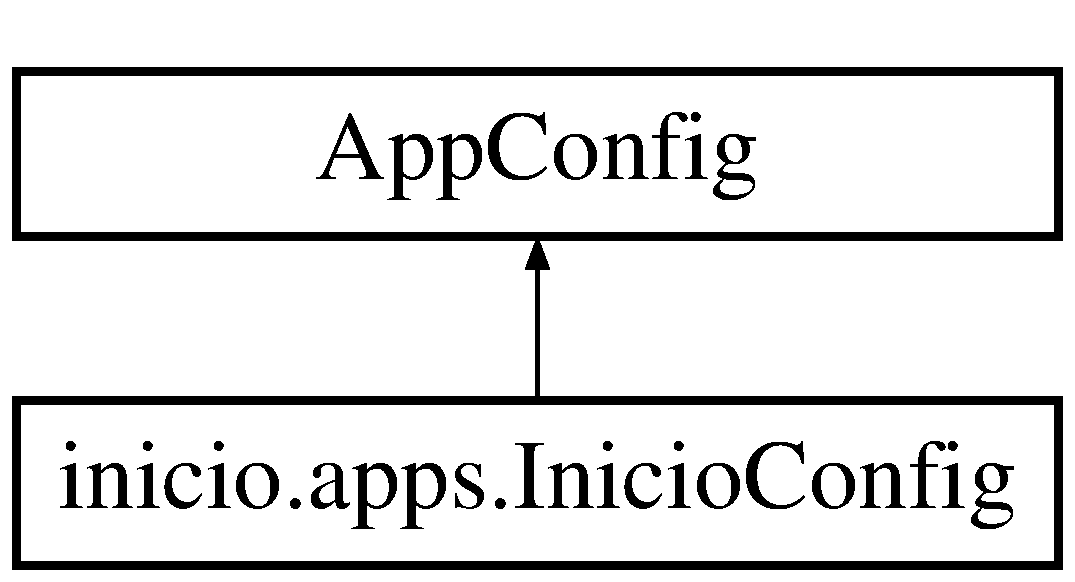
\includegraphics[height=2.000000cm]{classinicio_1_1apps_1_1_inicio_config}
\end{center}
\end{figure}
\subsection*{Static Public Attributes}
\begin{DoxyCompactItemize}
\item 
\mbox{\Hypertarget{classinicio_1_1apps_1_1_inicio_config_adf2662135be60120a99393a8211b1c92}\label{classinicio_1_1apps_1_1_inicio_config_adf2662135be60120a99393a8211b1c92}} 
string {\bfseries name} = \textquotesingle{}inicio\textquotesingle{}
\end{DoxyCompactItemize}


The documentation for this class was generated from the following file\+:\begin{DoxyCompactItemize}
\item 
F\+:/\+Git\+Hub/\+Projects/\+Asdecalidad-\/1/website/src/website/inicio/apps.\+py\end{DoxyCompactItemize}

\hypertarget{classinicio_1_1modelo_1_1muestra_1_1muestra}{}\section{inicio.\+modelo.\+muestra.\+muestra Class Reference}
\label{classinicio_1_1modelo_1_1muestra_1_1muestra}\index{inicio.\+modelo.\+muestra.\+muestra@{inicio.\+modelo.\+muestra.\+muestra}}
\subsection*{Public Member Functions}
\begin{DoxyCompactItemize}
\item 
\mbox{\Hypertarget{classinicio_1_1modelo_1_1muestra_1_1muestra_a402b8c8efcaea7d19d5d58b94e83dc6e}\label{classinicio_1_1modelo_1_1muestra_1_1muestra_a402b8c8efcaea7d19d5d58b94e83dc6e}} 
def {\bfseries \+\_\+\+\_\+init\+\_\+\+\_\+} (self)
\item 
def \hyperlink{classinicio_1_1modelo_1_1muestra_1_1muestra_aa851f3e02e1b300574d4b4e6d56584e9}{generar\+Matriz} (self)
\item 
\mbox{\Hypertarget{classinicio_1_1modelo_1_1muestra_1_1muestra_ae5af505ecfdd4abaea1e849fecf53aa2}\label{classinicio_1_1modelo_1_1muestra_1_1muestra_ae5af505ecfdd4abaea1e849fecf53aa2}} 
def {\bfseries generar\+Matriz\+Covarianza2} (self)
\item 
def \hyperlink{classinicio_1_1modelo_1_1muestra_1_1muestra_a395c113c5874b3f561737696d6658584}{generar\+Matriz\+Covarianza} (self)
\item 
def \hyperlink{classinicio_1_1modelo_1_1muestra_1_1muestra_aefb6a206689e6f0ff049028b68c5dc00}{calcular\+Autovalores} (self)
\item 
\mbox{\Hypertarget{classinicio_1_1modelo_1_1muestra_1_1muestra_ae57339075e6fc9ede255048d4ab9f945}\label{classinicio_1_1modelo_1_1muestra_1_1muestra_ae57339075e6fc9ede255048d4ab9f945}} 
def {\bfseries calcular\+Autovectores} (self)
\end{DoxyCompactItemize}
\subsection*{Public Attributes}
\begin{DoxyCompactItemize}
\item 
\mbox{\Hypertarget{classinicio_1_1modelo_1_1muestra_1_1muestra_ad1927a80cc26b0a4646714af1c2bf0cd}\label{classinicio_1_1modelo_1_1muestra_1_1muestra_ad1927a80cc26b0a4646714af1c2bf0cd}} 
{\bfseries sujetos}
\item 
\mbox{\Hypertarget{classinicio_1_1modelo_1_1muestra_1_1muestra_a057fea2d4c2b345581f6fae6e1176137}\label{classinicio_1_1modelo_1_1muestra_1_1muestra_a057fea2d4c2b345581f6fae6e1176137}} 
{\bfseries matriz}
\item 
\mbox{\Hypertarget{classinicio_1_1modelo_1_1muestra_1_1muestra_a6d0dc58bd3966414946e31e177fc2575}\label{classinicio_1_1modelo_1_1muestra_1_1muestra_a6d0dc58bd3966414946e31e177fc2575}} 
{\bfseries matriz\+Covarianza}
\item 
\mbox{\Hypertarget{classinicio_1_1modelo_1_1muestra_1_1muestra_ab3af3b7aecc0449f98d621e73aa78da1}\label{classinicio_1_1modelo_1_1muestra_1_1muestra_ab3af3b7aecc0449f98d621e73aa78da1}} 
{\bfseries autovalores}
\item 
\mbox{\Hypertarget{classinicio_1_1modelo_1_1muestra_1_1muestra_a1d86c1868968a8ef006ba084204b57fb}\label{classinicio_1_1modelo_1_1muestra_1_1muestra_a1d86c1868968a8ef006ba084204b57fb}} 
{\bfseries autovectores}
\end{DoxyCompactItemize}


\subsection{Detailed Description}
\begin{DoxyVerb}Encargada de representar y realizar calculos sobre las muestras 
\end{DoxyVerb}
 

\subsection{Member Function Documentation}
\mbox{\Hypertarget{classinicio_1_1modelo_1_1muestra_1_1muestra_aefb6a206689e6f0ff049028b68c5dc00}\label{classinicio_1_1modelo_1_1muestra_1_1muestra_aefb6a206689e6f0ff049028b68c5dc00}} 
\index{inicio\+::modelo\+::muestra\+::muestra@{inicio\+::modelo\+::muestra\+::muestra}!calcular\+Autovalores@{calcular\+Autovalores}}
\index{calcular\+Autovalores@{calcular\+Autovalores}!inicio\+::modelo\+::muestra\+::muestra@{inicio\+::modelo\+::muestra\+::muestra}}
\subsubsection{\texorpdfstring{calcular\+Autovalores()}{calcularAutovalores()}}
{\footnotesize\ttfamily def inicio.\+modelo.\+muestra.\+muestra.\+calcular\+Autovalores (\begin{DoxyParamCaption}\item[{}]{self }\end{DoxyParamCaption})}

\begin{DoxyVerb}Calcula los autovalores utilizando la matriz de covarianza.
\end{DoxyVerb}
 \mbox{\Hypertarget{classinicio_1_1modelo_1_1muestra_1_1muestra_aa851f3e02e1b300574d4b4e6d56584e9}\label{classinicio_1_1modelo_1_1muestra_1_1muestra_aa851f3e02e1b300574d4b4e6d56584e9}} 
\index{inicio\+::modelo\+::muestra\+::muestra@{inicio\+::modelo\+::muestra\+::muestra}!generar\+Matriz@{generar\+Matriz}}
\index{generar\+Matriz@{generar\+Matriz}!inicio\+::modelo\+::muestra\+::muestra@{inicio\+::modelo\+::muestra\+::muestra}}
\subsubsection{\texorpdfstring{generar\+Matriz()}{generarMatriz()}}
{\footnotesize\ttfamily def inicio.\+modelo.\+muestra.\+muestra.\+generar\+Matriz (\begin{DoxyParamCaption}\item[{}]{self }\end{DoxyParamCaption})}

\begin{DoxyVerb}Genera matriz de imagenes vectorizadas de cada sujeto
\end{DoxyVerb}
 \mbox{\Hypertarget{classinicio_1_1modelo_1_1muestra_1_1muestra_a395c113c5874b3f561737696d6658584}\label{classinicio_1_1modelo_1_1muestra_1_1muestra_a395c113c5874b3f561737696d6658584}} 
\index{inicio\+::modelo\+::muestra\+::muestra@{inicio\+::modelo\+::muestra\+::muestra}!generar\+Matriz\+Covarianza@{generar\+Matriz\+Covarianza}}
\index{generar\+Matriz\+Covarianza@{generar\+Matriz\+Covarianza}!inicio\+::modelo\+::muestra\+::muestra@{inicio\+::modelo\+::muestra\+::muestra}}
\subsubsection{\texorpdfstring{generar\+Matriz\+Covarianza()}{generarMatrizCovarianza()}}
{\footnotesize\ttfamily def inicio.\+modelo.\+muestra.\+muestra.\+generar\+Matriz\+Covarianza (\begin{DoxyParamCaption}\item[{}]{self }\end{DoxyParamCaption})}

\begin{DoxyVerb}Generacion de la matriz de covarianza para la definicion de informacion
relevante para los calculos
\end{DoxyVerb}
 

The documentation for this class was generated from the following file\+:\begin{DoxyCompactItemize}
\item 
F\+:/\+Git\+Hub/\+Projects/\+Asdecalidad-\/1/website/src/website/inicio/modelo/muestra.\+py\end{DoxyCompactItemize}

\hypertarget{classinicio_1_1controlador_1_1controlador_1_1sujeto}{}\section{inicio.\+controlador.\+controlador.\+sujeto Class Reference}
\label{classinicio_1_1controlador_1_1controlador_1_1sujeto}\index{inicio.\+controlador.\+controlador.\+sujeto@{inicio.\+controlador.\+controlador.\+sujeto}}
\subsection*{Public Member Functions}
\begin{DoxyCompactItemize}
\item 
\mbox{\Hypertarget{classinicio_1_1controlador_1_1controlador_1_1sujeto_a038d0ffbccc3cebebd62399b2dedbf24}\label{classinicio_1_1controlador_1_1controlador_1_1sujeto_a038d0ffbccc3cebebd62399b2dedbf24}} 
def {\bfseries \+\_\+\+\_\+init\+\_\+\+\_\+} (self)
\item 
\mbox{\Hypertarget{classinicio_1_1controlador_1_1controlador_1_1sujeto_ae39c95a044b8a11fdb2247e2d92a12e7}\label{classinicio_1_1controlador_1_1controlador_1_1sujeto_ae39c95a044b8a11fdb2247e2d92a12e7}} 
def {\bfseries leer\+Carpetas} (self)
\item 
\mbox{\Hypertarget{classinicio_1_1controlador_1_1controlador_1_1sujeto_a7380175285a8bf3bb1483634bde13097}\label{classinicio_1_1controlador_1_1controlador_1_1sujeto_a7380175285a8bf3bb1483634bde13097}} 
def {\bfseries leer\+Imagenes} (self)
\end{DoxyCompactItemize}
\subsection*{Public Attributes}
\begin{DoxyCompactItemize}
\item 
\mbox{\Hypertarget{classinicio_1_1controlador_1_1controlador_1_1sujeto_a7a99e4c46254bf3e76a991ba38a1da20}\label{classinicio_1_1controlador_1_1controlador_1_1sujeto_a7a99e4c46254bf3e76a991ba38a1da20}} 
{\bfseries vector}
\end{DoxyCompactItemize}


The documentation for this class was generated from the following file\+:\begin{DoxyCompactItemize}
\item 
F\+:/\+Git\+Hub/\+Projects/\+Asdecalidad-\/1/website/src/website/inicio/controlador/controlador.\+py\end{DoxyCompactItemize}

\hypertarget{classinicio_1_1modelo_1_1sujeto_1_1sujeto}{}\section{inicio.\+modelo.\+sujeto.\+sujeto Class Reference}
\label{classinicio_1_1modelo_1_1sujeto_1_1sujeto}\index{inicio.\+modelo.\+sujeto.\+sujeto@{inicio.\+modelo.\+sujeto.\+sujeto}}
\subsection*{Public Member Functions}
\begin{DoxyCompactItemize}
\item 
def \hyperlink{classinicio_1_1modelo_1_1sujeto_1_1sujeto_adc5fdb70533f566da487a316f753a0e8}{\+\_\+\+\_\+init\+\_\+\+\_\+} (self, nombre)
\item 
def \hyperlink{classinicio_1_1modelo_1_1sujeto_1_1sujeto_a6f4b6d7118b152c714e87d5c7e38d60a}{agregar\+Imagene} (self, \hyperlink{classinicio_1_1modelo_1_1imagen_1_1imagen}{imagen})
\end{DoxyCompactItemize}
\subsection*{Public Attributes}
\begin{DoxyCompactItemize}
\item 
\mbox{\Hypertarget{classinicio_1_1modelo_1_1sujeto_1_1sujeto_ac67e083c0bbdd0266c6d16d70e481199}\label{classinicio_1_1modelo_1_1sujeto_1_1sujeto_ac67e083c0bbdd0266c6d16d70e481199}} 
{\bfseries nombre}
\item 
\mbox{\Hypertarget{classinicio_1_1modelo_1_1sujeto_1_1sujeto_a20cee61c3e73eb44582e2a14720dd467}\label{classinicio_1_1modelo_1_1sujeto_1_1sujeto_a20cee61c3e73eb44582e2a14720dd467}} 
{\bfseries imagenes}
\item 
\mbox{\Hypertarget{classinicio_1_1modelo_1_1sujeto_1_1sujeto_aa0f06102e3b69e1820ab6192926eae54}\label{classinicio_1_1modelo_1_1sujeto_1_1sujeto_aa0f06102e3b69e1820ab6192926eae54}} 
{\bfseries matriz}
\end{DoxyCompactItemize}


\subsection{Detailed Description}
\begin{DoxyVerb}Clase encargada de representar a los sujetos a quienes pertenecen las imagenes.
\end{DoxyVerb}
 

\subsection{Constructor \& Destructor Documentation}
\mbox{\Hypertarget{classinicio_1_1modelo_1_1sujeto_1_1sujeto_adc5fdb70533f566da487a316f753a0e8}\label{classinicio_1_1modelo_1_1sujeto_1_1sujeto_adc5fdb70533f566da487a316f753a0e8}} 
\index{inicio\+::modelo\+::sujeto\+::sujeto@{inicio\+::modelo\+::sujeto\+::sujeto}!\+\_\+\+\_\+init\+\_\+\+\_\+@{\+\_\+\+\_\+init\+\_\+\+\_\+}}
\index{\+\_\+\+\_\+init\+\_\+\+\_\+@{\+\_\+\+\_\+init\+\_\+\+\_\+}!inicio\+::modelo\+::sujeto\+::sujeto@{inicio\+::modelo\+::sujeto\+::sujeto}}
\subsubsection{\texorpdfstring{\+\_\+\+\_\+init\+\_\+\+\_\+()}{\_\_init\_\_()}}
{\footnotesize\ttfamily def inicio.\+modelo.\+sujeto.\+sujeto.\+\_\+\+\_\+init\+\_\+\+\_\+ (\begin{DoxyParamCaption}\item[{}]{self,  }\item[{}]{nombre }\end{DoxyParamCaption})}

\begin{DoxyVerb}Constructor
:param nombre: Nombre del sujeto.
\end{DoxyVerb}
 

\subsection{Member Function Documentation}
\mbox{\Hypertarget{classinicio_1_1modelo_1_1sujeto_1_1sujeto_a6f4b6d7118b152c714e87d5c7e38d60a}\label{classinicio_1_1modelo_1_1sujeto_1_1sujeto_a6f4b6d7118b152c714e87d5c7e38d60a}} 
\index{inicio\+::modelo\+::sujeto\+::sujeto@{inicio\+::modelo\+::sujeto\+::sujeto}!agregar\+Imagene@{agregar\+Imagene}}
\index{agregar\+Imagene@{agregar\+Imagene}!inicio\+::modelo\+::sujeto\+::sujeto@{inicio\+::modelo\+::sujeto\+::sujeto}}
\subsubsection{\texorpdfstring{agregar\+Imagene()}{agregarImagene()}}
{\footnotesize\ttfamily def inicio.\+modelo.\+sujeto.\+sujeto.\+agregar\+Imagene (\begin{DoxyParamCaption}\item[{}]{self,  }\item[{}]{imagen }\end{DoxyParamCaption})}

\begin{DoxyVerb}Agrega una imagen a la lista de imagenes del sujeto.
:param imagen: Imagen a agregar.
\end{DoxyVerb}
 

The documentation for this class was generated from the following file\+:\begin{DoxyCompactItemize}
\item 
F\+:/\+Git\+Hub/\+Projects/\+Asdecalidad-\/1/website/src/website/inicio/modelo/sujeto.\+py\end{DoxyCompactItemize}

\hypertarget{classtest_cases_1_1test_cases}{}\section{test\+Cases.\+test\+Cases Class Reference}
\label{classtest_cases_1_1test_cases}\index{test\+Cases.\+test\+Cases@{test\+Cases.\+test\+Cases}}
Inheritance diagram for test\+Cases.\+test\+Cases\+:\begin{figure}[H]
\begin{center}
\leavevmode
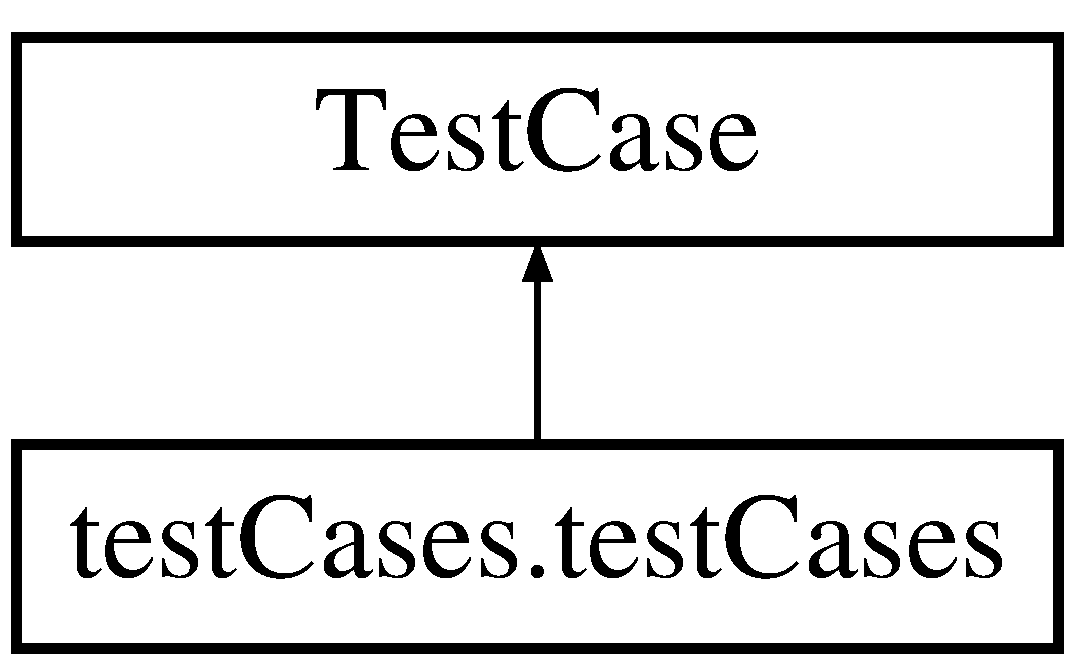
\includegraphics[height=2.000000cm]{classtest_cases_1_1test_cases}
\end{center}
\end{figure}
\subsection*{Public Member Functions}
\begin{DoxyCompactItemize}
\item 
\mbox{\Hypertarget{classtest_cases_1_1test_cases_aa979286944bac3542084f99f45ddd45b}\label{classtest_cases_1_1test_cases_aa979286944bac3542084f99f45ddd45b}} 
def {\bfseries test\+Cargar\+Desde\+BD} (self)
\item 
\mbox{\Hypertarget{classtest_cases_1_1test_cases_a6f02655300cb85c1ff3b3b8f5921f0a1}\label{classtest_cases_1_1test_cases_a6f02655300cb85c1ff3b3b8f5921f0a1}} 
def {\bfseries test\+Generar\+Matriz\+Imagenes} (self)
\item 
\mbox{\Hypertarget{classtest_cases_1_1test_cases_a30fc99af58abaf329f8ce70d41273f7a}\label{classtest_cases_1_1test_cases_a30fc99af58abaf329f8ce70d41273f7a}} 
def {\bfseries test\+Cambiar\+Tamano} (self)
\item 
\mbox{\Hypertarget{classtest_cases_1_1test_cases_a59a34e3f0fc3f26697cfedcca798968a}\label{classtest_cases_1_1test_cases_a59a34e3f0fc3f26697cfedcca798968a}} 
def {\bfseries test\+Matriz\+Covarianza} (self)
\end{DoxyCompactItemize}


\subsection{Detailed Description}
\begin{DoxyVerb}Clase destinada a la ejecucion de pruebas unittest
\end{DoxyVerb}
 

The documentation for this class was generated from the following file\+:\begin{DoxyCompactItemize}
\item 
F\+:/\+Git\+Hub/\+Projects/\+Asdecalidad-\/1/website/src/website/inicio/tests/test\+Cases.\+py\end{DoxyCompactItemize}

\hypertarget{classinicio_1_1forms_1_1_upload_file_form}{}\section{inicio.\+forms.\+Upload\+File\+Form Class Reference}
\label{classinicio_1_1forms_1_1_upload_file_form}\index{inicio.\+forms.\+Upload\+File\+Form@{inicio.\+forms.\+Upload\+File\+Form}}
Inheritance diagram for inicio.\+forms.\+Upload\+File\+Form\+:\begin{figure}[H]
\begin{center}
\leavevmode
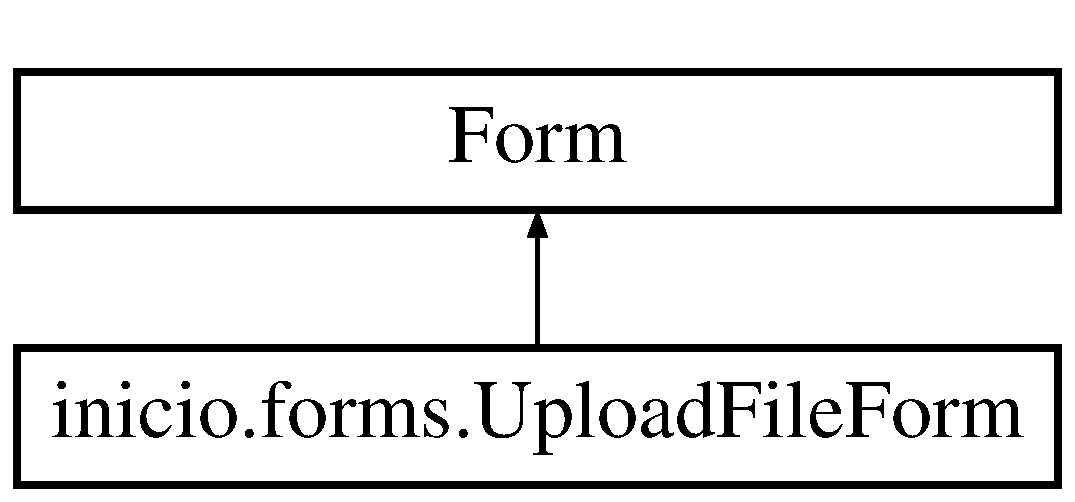
\includegraphics[height=2.000000cm]{classinicio_1_1forms_1_1_upload_file_form}
\end{center}
\end{figure}


The documentation for this class was generated from the following file\+:\begin{DoxyCompactItemize}
\item 
F\+:/\+Git\+Hub/\+Projects/\+Asdecalidad-\/1/website/src/website/inicio/forms.\+py\end{DoxyCompactItemize}

%--- End generated contents ---

% Index
\backmatter
\newpage
\phantomsection
\clearemptydoublepage
\addcontentsline{toc}{chapter}{Index}
\printindex

\end{document}
